\documentclass[12pt,a4paper]{article}

% inputenc omitted: utf8 engines load it by default
\usepackage[T1]{fontenc}
\usepackage{amsmath,amssymb,amsfonts}
\usepackage{amsthm}
\usepackage{graphicx}
\usepackage{booktabs}
\usepackage{hyperref}
\usepackage{xcolor}
\usepackage[margin=2.5cm]{geometry}
\usepackage{setspace}
\usepackage{natbib}
\usepackage{caption}
\usepackage{subcaption}
\usepackage{float}
\usepackage{siunitx}
\usepackage{tikz}
\usetikzlibrary{arrows.meta, positioning}
\usepackage[expansion=false]{microtype}   % expansion disabled: MiKTeX bitmap font fallback
\usepackage{xr}
% seqsplit not needed (long numbers handled inline)

% The supplementary document carries the moved derivations and supporting floats;
% their labels resolve here so that a citation of a supplementary item prints its
% S-number. The guard keeps a single-document build from failing.
\IfFileExists{build_v2/supplementary_text.aux}
  {\externaldocument{build_v2/supplementary_text}}{}

\captionsetup{justification=raggedright, singlelinecheck=false}

\onehalfspacing
\emergencystretch=2em   % keeps inline formulas from spilling past the margins
\bibliographystyle{apalike}   % single declaration

% Commandes personnelles
\newcommand{\Rey}{\mathit{Re}}
\newcommand{\Pe}{\mathit{Pe}}
\newcommand{\Grr}{\mathit{Gr}}
\newcommand{\Nu}{\mathit{Nu}}
\renewcommand{\Pr}{\mathit{Pr}}

\newcommand{\PiT}{\Pi_T}

\newtheorem{theorem}{Theorem}
\newtheorem{proposition}{Proposition}
\newtheorem{corollary}{Corollary}
\newtheorem{lemma}{Lemma}
\newenvironment{acknowledgments}{\section*{Acknowledgments}}{}
\newenvironment{ruledtabular}{}{}

\begin{document}

\title{\textbf{Symmetry-Selected Nonlinear Thermal Pumping in
       Periodically Heated Mixed-Convection Channels}}
\author{BENIAICHE Ahmed \\
\textit{Laboratory of Fluid Mechanics, Ecole Militaire Polytechnique,} \\
\textit{Algiers, Algeria} \\
\textit{Email: beniaiche\_ahmed25@yahoo.fr}}
\date{}
\maketitle

\begin{abstract}
Nonlinear redistribution of wall heat flux in a two-dimensional laminar
mixed-convection channel with spatially periodic wall-temperature modulation of
unequal amplitude is governed by an exact symmetry selection rule, while the
magnitude and the direction of the redistribution are set by the coupled
thermal--hydrodynamic dynamics. Decomposing the first-order thermal response into
symmetric and antisymmetric Fourier components, we prove that their mixed quadratic
interaction is odd across the channel, so that the second-order mean wall-flux
corrections satisfy $\Nu_{2,0}(+1)=-\Nu_{2,0}(-1)$ identically, whereas
symmetry-preserving self-interactions produce no directional redistribution at the
same order. The parity law defines a thermal-pumping coefficient $\PiT$ that obeys
the exact Green-function identity $\PiT=-(\Pe/2)\int_{-1}^{1}Y\mathcal E_{as}\,dY$,
from which the linearity $\PiT=\Grr A(k,\Rey,\Pr)$, the long-wavelength scaling
$A=O(k^2)$, and the corollary that the zero of $\PiT$ is independent of $\Grr$ all
follow. An independent fully nonlinear DNS, at $(k,\Pe,\Rey,\Pr,\Grr)$ equal to
$(0.8,7,10,0.7,100)$, converges to
$\PiT^{\mathrm{DNS}}=-4.6763\times10^{-2}$, within $1.52\%$ of the perturbative
prediction, reproduces the symmetry-selected reversal upon interchange of the two
wall amplitudes, and confirms that the reversal point in $\Rey$ does not move when
$\Grr$ is varied over $25$--$200$. At fixed $\Pe$ the reversal location
$\Rey_c(k)$ is mapped perturbatively over seven wavenumbers, from
$\Rey_c=79.08$ at $k=0.4$ to $\Rey_c=8.54$ at $k=2.0$. A thirteen-case DNS
campaign then confirms the reversal nonlinearly on both sides of the crossing at
four wavenumbers, all eight bracketed cases returning the predicted sign,
reproduces the parity cancellation to $3.1\times10^{-18}$ in the wall-flux
difference, measures the quadrature coefficient to $1.38\%$, and extends the
Grashof-independence of the reversal to the nonlinear regime: the measured
Grashof ratios of $q_+-q_-$ lie within $3.7\times10^{-4}$ of the exact factor of
four and the DNS-minus-perturbative discrepancy is itself proportional to
$\Grr$, so the discrepancy rescales the coefficient without moving its zero.
The same campaign falsifies part of its own pre-registered error model---five of
the twelve non-degenerate cases exceed the bound, with a deviation independent
of the forcing amplitude and growing with the wavenumber---and the residual is
analysed as a remainder whose origin, truncation or spatial discretisation, is
not separated. The parity law is shown
to extend to phase-shifted forcing through a second, independent pumping
coefficient $\PiT^{\perp}$ that enters with the quadrature product
$\mathrm{Im}(\varepsilon_a\varepsilon_s^{*})$ and reverses the pumping direction on
its own. Symmetry therefore selects the \emph{structure} of the nonlinear
redistribution, whereas buoyancy-mediated dynamics select its amplitude, its sign,
and the control parameter that governs it.
\end{abstract}

\noindent\textbf{Keywords:} mixed convection; streamwise-periodic wall heating;
thermal pumping; symmetry selection rule; weakly nonlinear expansion;
Reynolds-number reversal; direct numerical simulation; reproducibility

%--------------------------------------------------------------
\section*{Nomenclature}
\label{sec:nomenclature}
%--------------------------------------------------------------
\begin{table}[htb]
\begin{ruledtabular}
\begin{tabular}{ll}
\textbf{Roman Symbols} & \\
$A(k,\Rey,\Pr)$ & Normalized pumping response, $A=\PiT/\Grr$ [-] \\
$H$ & Channel half-width [m] \\
$k$ & Dimensionless modulation wavenumber [-] \\
$k^*$ & Zero of $\PiT(k,\Pe)$ when an interior crossing exists [-] \\
$\Nu$ & Nusselt number [-] \\
$p$ & Pressure [Pa] \\
$\Pe$ & P\'eclet number, $\Pe=\Rey\Pr$ [-] \\
$\Pr$ & Prandtl number, $\Pr=\nu/\alpha$ [-] \\
$\Grr$ & Grashof number, $\Grr=g\beta\Delta T H^3/\nu^2$ [-] \\
$\Rey$ & Reynolds number, $\Rey=U_0H/\nu$ [-] \\
$U_0$ & Reference mean velocity used for nondimensionalization [m/s] \\
$X,Y$ & Dimensionless streamwise and transverse coordinates [-] \\
\textbf{Greek Symbols} & \\
$\alpha$ & Thermal diffusivity [m$^2$/s] \\
$\beta$ & Thermal expansion coefficient [K$^{-1}$] \\
$\varepsilon_1,\varepsilon_2$ & Dimensionless wall-modulation amplitudes [-] \\
$\varepsilon_s,\varepsilon_a$ & Symmetric and antisymmetric amplitudes [-] \\
$\theta$ & Dimensionless temperature perturbation [-] \\
$\nu$ & Kinematic viscosity [m$^2$/s] \\
$\PiT$ & Normalized nonlinear thermal pumping coefficient [-] \\
$\phi$ & Phase shift between wall modulations [rad] \\
\textbf{Abbreviations} & \\
BC & Boundary condition \\
BVP & Boundary-value problem \\
IVP & Initial-value problem \\
RK & Runge--Kutta \\
\end{tabular}
\end{ruledtabular}
\end{table}

%--------------------------------------------------------------
\section{Introduction}
%--------------------------------------------------------------

Two mechanisms are deliberately separated throughout this paper. Reflection
\emph{symmetry} selects the \emph{structure} of the nonlinear redistribution of the
wall heat flux: the second-order mean corrections at the two walls are exactly equal
in magnitude and opposite in sign. The thermal--hydrodynamic \emph{dynamics} select
the \emph{amplitude and the sign} of that redistribution, and at fixed P\'eclet
number the Reynolds number controls the direction of the pumping. Every result below
is assigned to one of these two categories, and the central claim of the paper is
that the division is exact rather than rhetorical: the first statement holds as a
theorem under stated assumptions, whereas the second requires quantitative
calculation and can even reverse.

Mixed convection in vertical channels is a classical problem in which imposed shear and buoyancy
interact to modify the velocity, temperature, and heat-transfer fields. Early analyses established
the fully developed theory and the possibility of buoyancy-induced flow reversal in vertical parallel-
plate channels \cite{AungWorku1986Theory,AungWorku1986Developing,HamadahWirtz1991}, while subsequent
work considered asymmetric wall heating and its effect on the hydrodynamic and thermal response
\cite{AungWorku1987,Barletta1998,Barletta1999}. These studies provide the mixed-convection foundation
for the present analysis.

Spatially periodic thermal forcing introduces a separate mechanism: the wall temperature varies along
the streamwise direction and generates thermal modes that interact with the base flow and, through
buoyancy, with perturbation velocities. Periodically heated channels have been investigated both for
natural convection and mixed convection, including vertical-channel configurations with spatially
periodic wall temperatures \cite{Dritselis2013,HossainFloryan2015}. The present problem is distinct in
that the central observable is not an instability threshold or a global heat-transfer enhancement,
but a second-order redistribution of the mean wall heat flux caused by deliberate breaking of the
reflection symmetry between the two walls.

The word \emph{pumping} requires a qualification, because it is used in the literature for a
different device. Thermal-wave pumping produces a net mean flow by means of a temperature wave
travelling along the boundary \cite{HossainFloryan2023}; the present rectified quantity is not a
propulsive flux but the difference between the two wall heat fluxes, i.e.\ a redistribution of heat
across the channel at strictly fixed bulk flow rate. The mechanisms are also unrelated: there the
asymmetry is imposed by a propagating phase, here it is imposed by the parity of a standing
quadratic interaction between a symmetric and an antisymmetric thermal mode.

Weakly nonlinear expansions are a natural tool for identifying such rectified responses. In hydrodynamic
stability theory, nonlinear interactions between Fourier modes and the associated mean-flow corrections
form a standard framework \cite{Stuart1960}; symmetry and mode selection are likewise central to the
broader theory of pattern-forming systems \cite{CrossHohenberg1993}. Here, however, the reference state
is not studied as an instability threshold. The weakly nonlinear expansion is used to expose an exact
symmetry selection rule embedded in the steady forced transport problem.

For identical upper and lower wall modulations, $\varepsilon_1=\varepsilon_2$, the leading second-order
wall-flux redistribution is symmetry-forbidden. The corresponding nonlinear forcing is even in the
transverse coordinate and cannot generate a persistent difference between the two inward wall heat
fluxes. The symmetric configuration therefore supplies a precise baseline against which the effect of
structural asymmetry can be isolated.

The present study asks what happens when $\varepsilon_1\neq\varepsilon_2$. We answer this question at
two levels. First, reflection symmetry and uniqueness produce an exact selection rule: the mixed
symmetric--antisymmetric interaction is odd in the transverse coordinate, and therefore its second-order
wall-flux corrections are equal in magnitude and opposite in sign. Second, the amplitude and sign of
this redistribution are determined by the coupled thermal and hydrodynamic response and hence remain
parameter dependent. This distinction is central: wall-flux antisymmetry is exact under the stated
assumptions, whereas nonzero pumping, its $k\to0$ scaling, and the location of its zero crossing are
dynamical results requiring quantitative calculation.

The contributions of the paper are therefore threefold.
\begin{enumerate}
  \item An \textbf{exact symmetry-selection theorem} (Theorem~\ref{thm:symmetry}): the mixed
  symmetric--antisymmetric second-order forcing is odd, hence
  $\Nu_{2,0}(+1)=-\Nu_{2,0}(-1)$ for every admissible $(\Rey,\Pr,\Grr,k)$, and pure
  symmetric or pure antisymmetric heating produce no directional redistribution at
  this order.
  \item An \textbf{exact two-coefficient phase law} (Proposition~2): for
  phase-shifted wall modulation the rectified wall-flux response is governed by the
  real and imaginary parts of the product $\varepsilon_a\varepsilon_s^{*}$, each
  multiplying an independent pumping coefficient. For equal wall amplitudes the
  dependence on the phase is exactly $\sin\phi$, with no higher harmonic, and the
  quadrature coefficient $\PiT^{\perp}$ has the \emph{opposite sign} to the
  published in-phase coefficient $\PiT$.
  \item A \textbf{dynamical mapping of the reversal}, validated by fully nonlinear
  DNS: the parity cancellation itself is reproduced in DNS to
  $3.1\times10^{-18}$ in the wall-flux difference, which is
  $2.7\times10^{-11}$ of the flux measured; the reversal point $\Rey_c$ at fixed
  $\Pe$ is independent of $\Grr$ to $1.2\times10^{-10}$ perturbatively and keeps
  its sign across a Grashof pair in DNS; the locus is mapped as a function of
  $k$ and confirmed on both sides of four of its crossings; and a term-wise
  phase analysis identifies which nonlinear
  transport contribution loses the balance as $\Rey$ increases.
\end{enumerate}
What is deliberately \emph{not} claimed is universality: the results are two-dimensional,
laminar, and restricted to the parameter domain where the second-order expansion is
quantitatively controlled.

\paragraph{Relation to the companion studies.}
This paper is the third and symmetry-selecting member of a series on the same canonical
configuration. The first study treats the \emph{symmetric} wall modulation and develops the exact
integral framework for the first-order complex thermal amplitude, including the non-monotonic
k-dependence of the mode-coupling coefficient. The second study treats the same symmetric problem
with a corrected modal decomposition and a fourth-order hydrodynamic boundary-value problem, and
establishes that $\Nu_{2,0}=0$ in that configuration, together with the three-regime map of the
first-order response. The present study changes the object of interest: it is the asymmetric
configuration, the exact parity selection rule that follows from it, and the dynamical
consequences of that rule. Only the shared canonical geometry and the standard nondimensional
Navier--Stokes--Boussinesq statement appear again; no derivation, table or figure of the
companion studies is reproduced here. Neither companion manuscript has yet appeared in print or
on a preprint server, so neither carries a citable identifier; they are therefore described in
the text rather than cited in the reference list, and are supplied to the editor on request.
Fig.~\ref{fig:schematic_geometry} shows the configuration and the two parity classes of wall
modulation it makes accessible, and Fig.~\ref{fig:logic_diagram} traces the chain from wall
symmetry to the admissible second-order response.

\begin{figure}[htb]
  \centering
  \begin{subfigure}{0.49\textwidth}
    \centering
    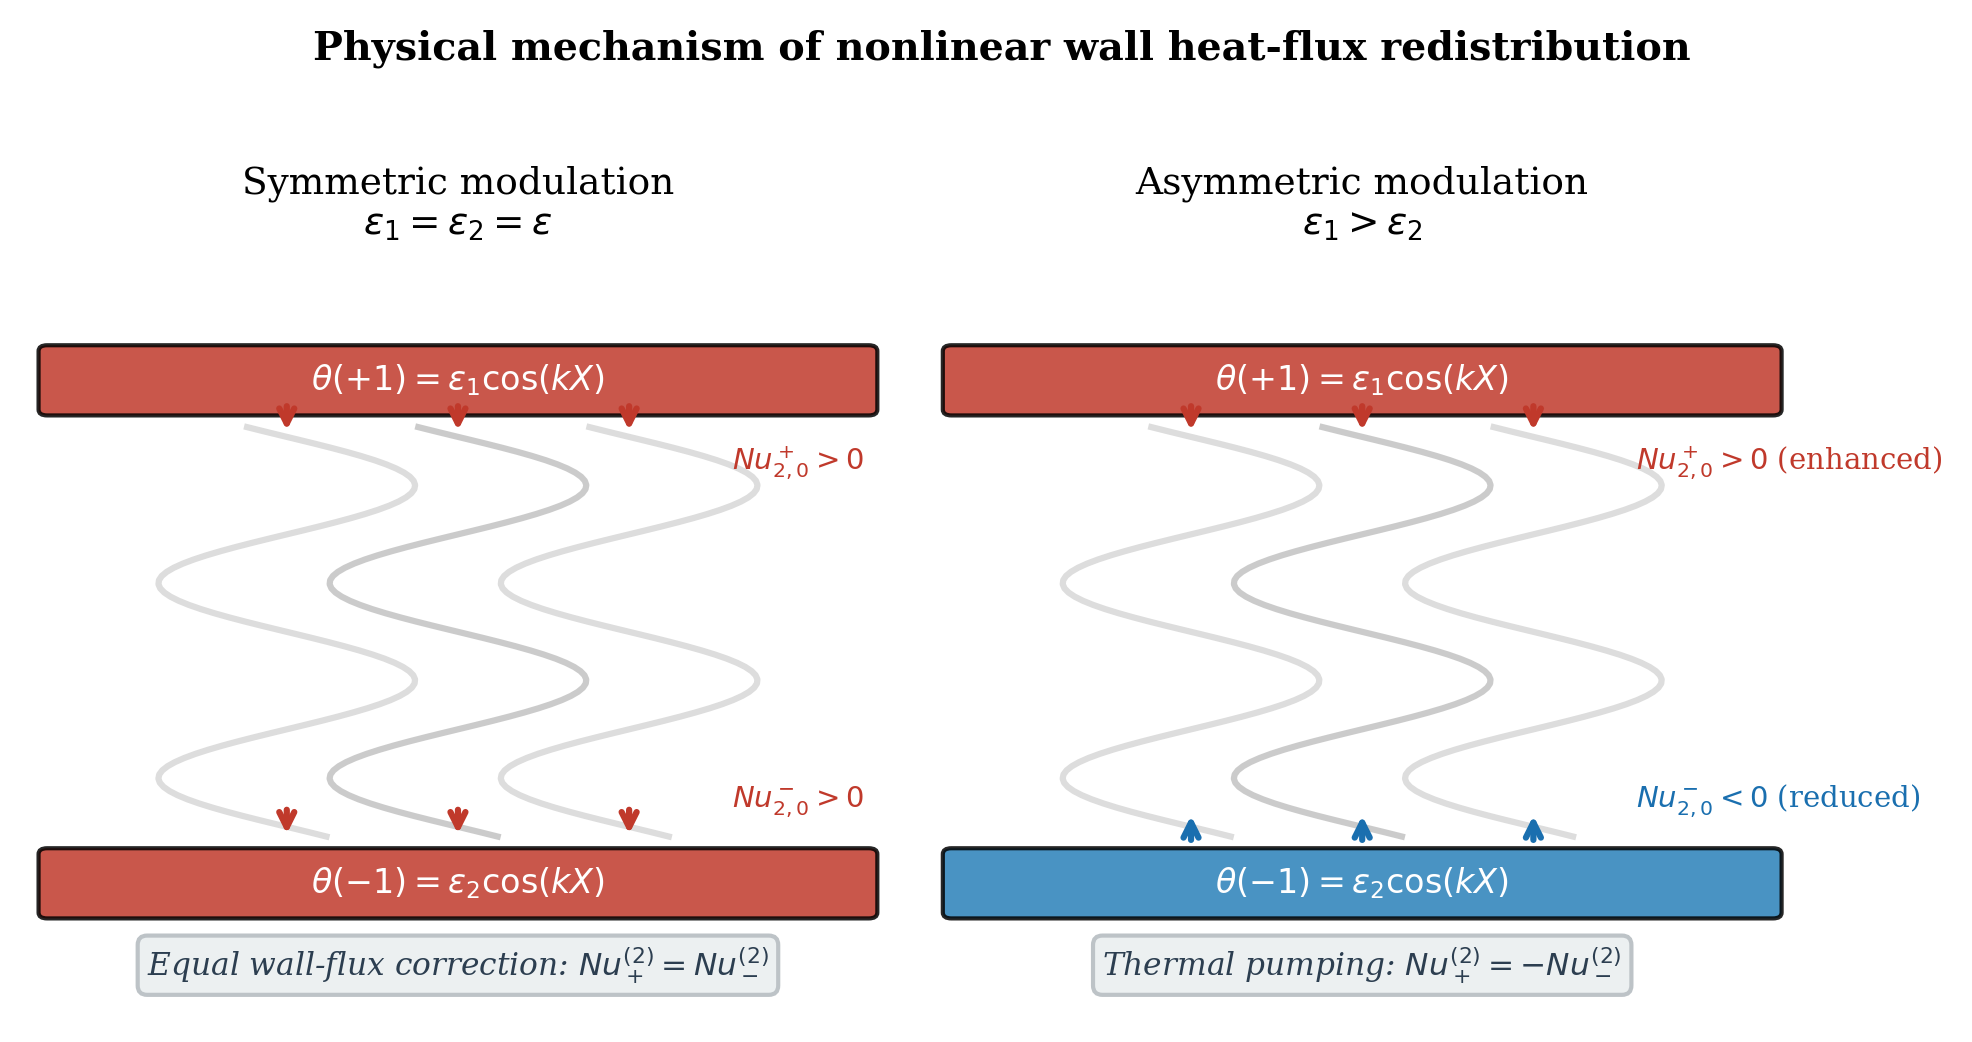
\includegraphics[width=\textwidth]{fig00_schematic.png}
    \caption{Mechanism: symmetric versus unequal wall amplitudes.}
    \label{fig:schematic}
  \end{subfigure}\hfill
  \begin{subfigure}{0.49\textwidth}
    \centering
    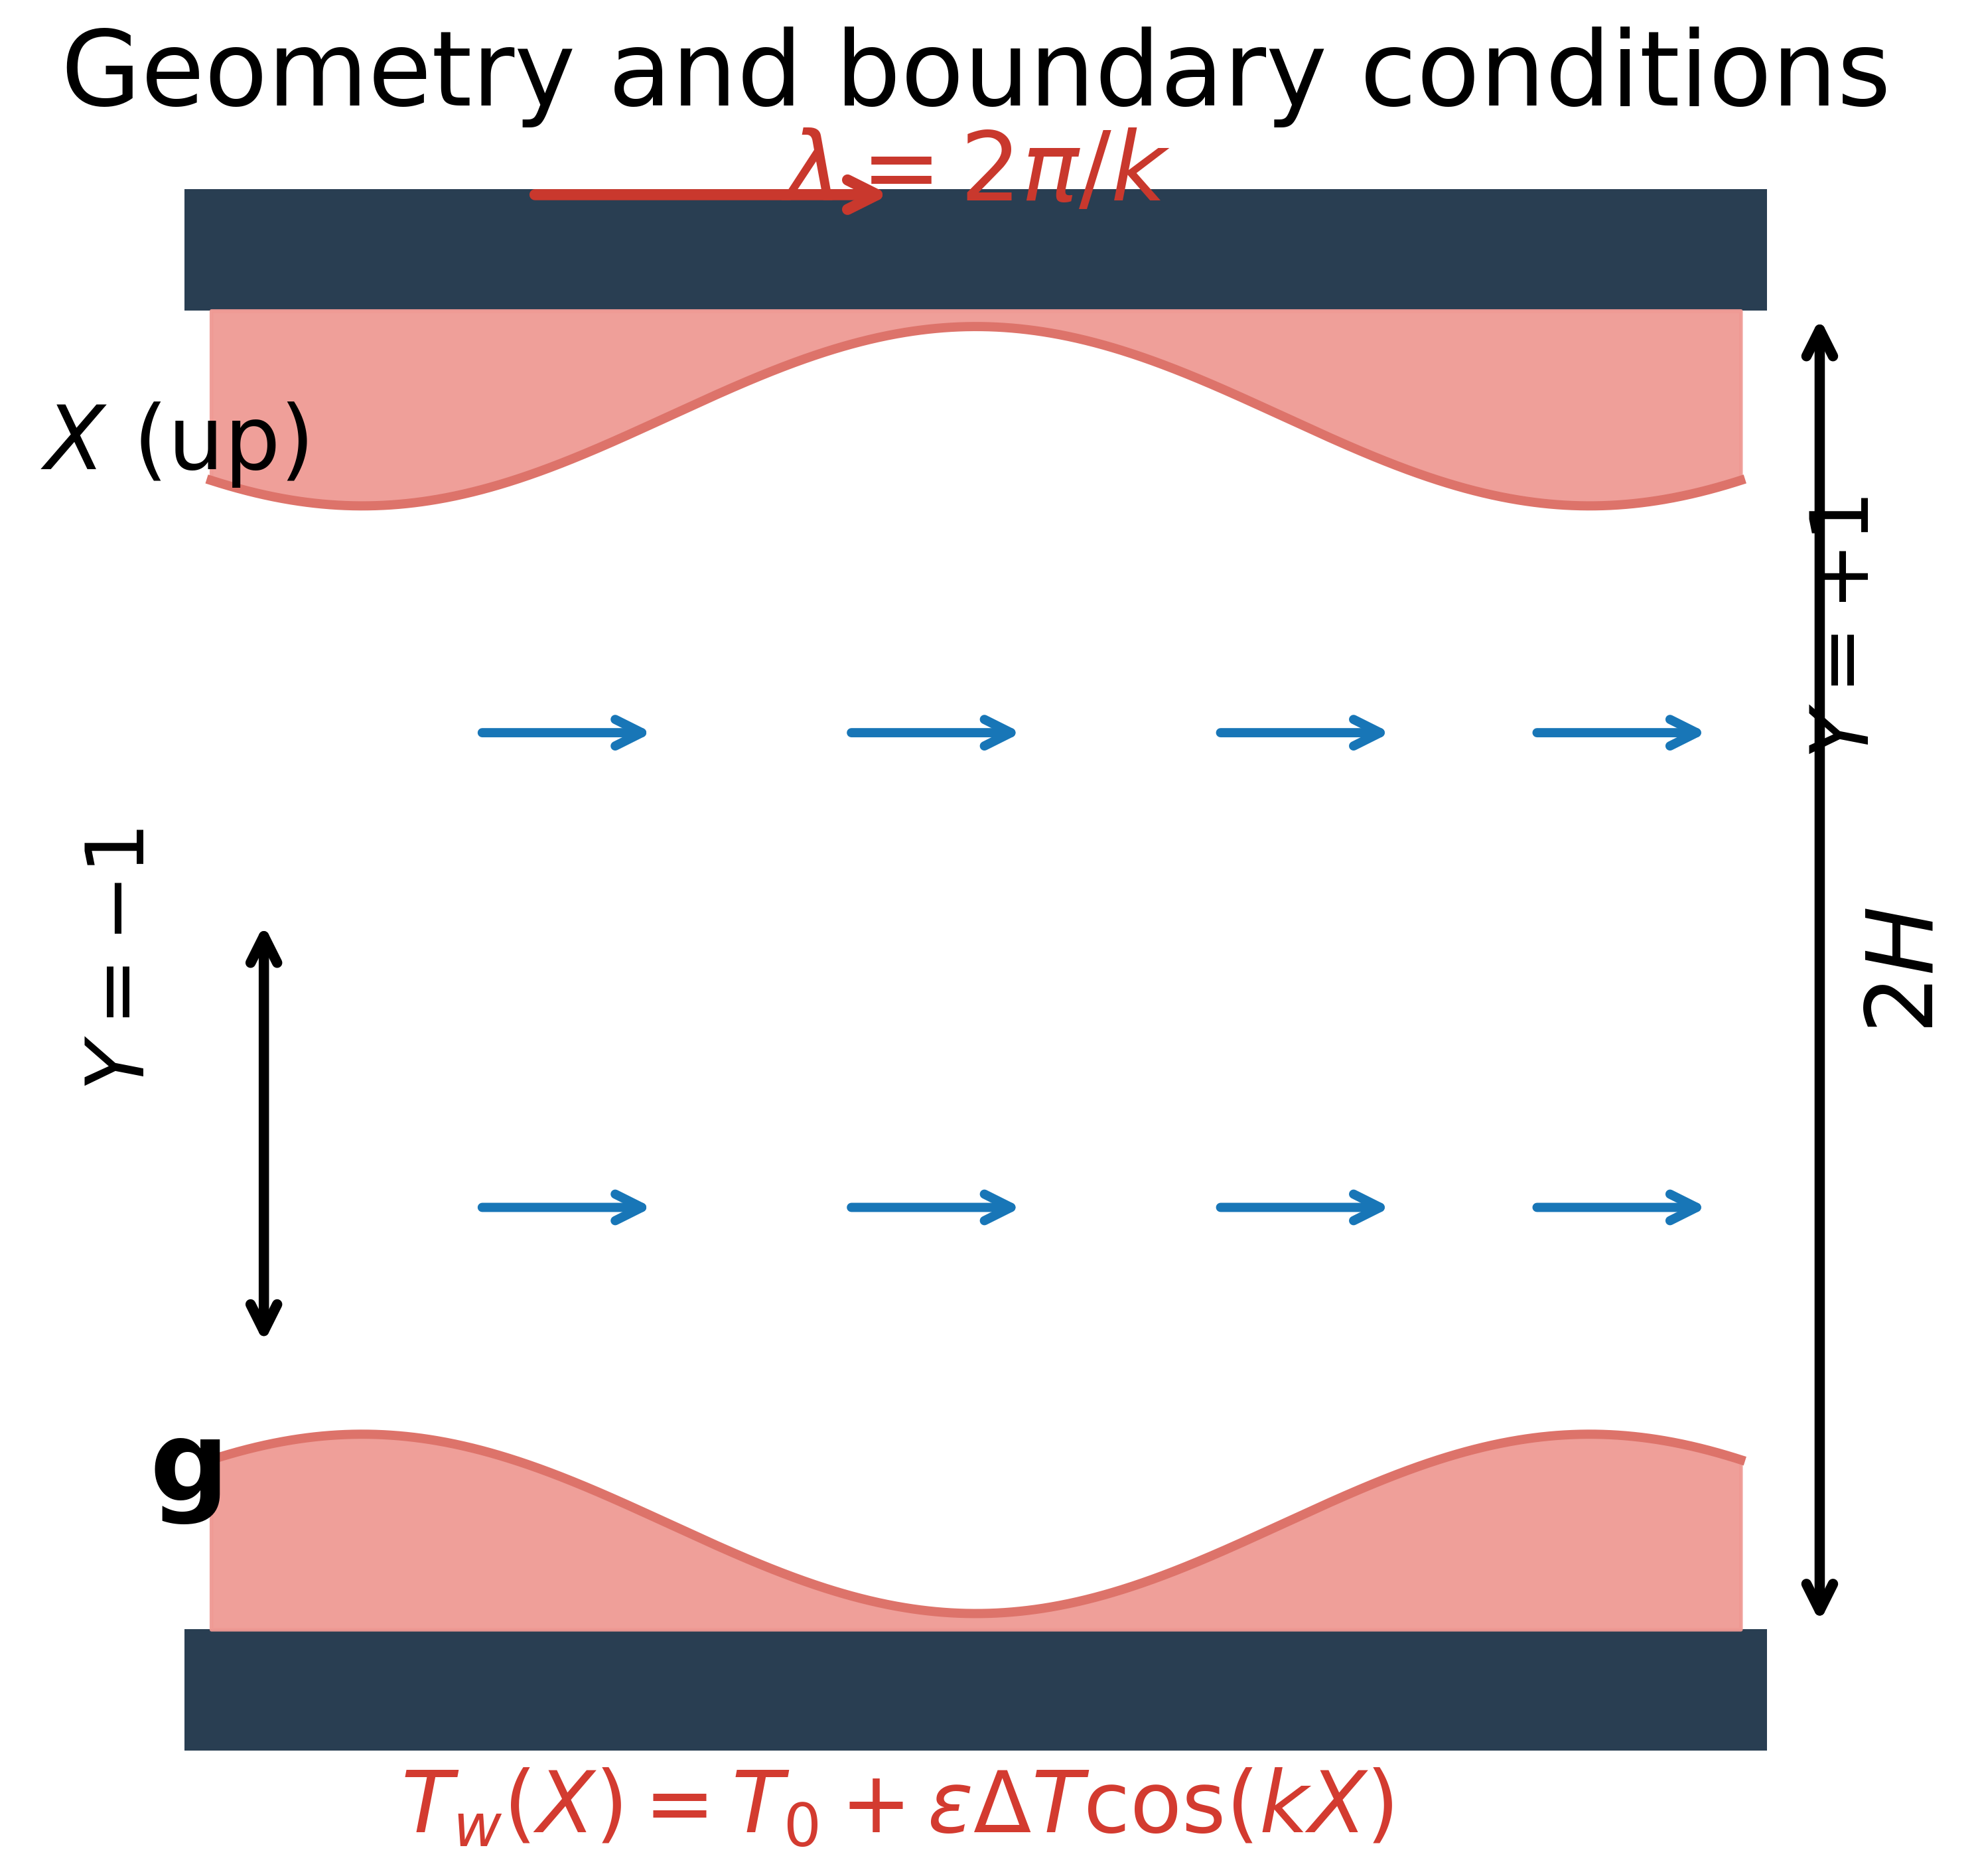
\includegraphics[width=\textwidth]{fig01_geometry.png}
    \caption{Geometry, base flow and nondimensionalization.}
    \label{fig:geometry}
  \end{subfigure}
  \caption{Physical schematic of the wall heat-flux redistribution mechanism and the
  configuration on which it acts. The symmetric limit suppresses the antisymmetric
  wall-flux correction, whereas unequal wall-modulation amplitudes activate the mixed
  symmetric--antisymmetric interaction responsible for the second-order redistribution.
  The vertical channel has walls at $Y=\pm1$, half-width $H$, base Poiseuille flow
  $U_0(Y)=\tfrac32(1-Y^2)$, gravity in the vertical direction, and periodically
  modulated wall temperatures with amplitudes $\varepsilon_1$ and $\varepsilon_2$.}
  \label{fig:schematic_geometry}
\end{figure}

%--------------------------------------------------------------
\section{Formulation and Base State}
%--------------------------------------------------------------

A laminar, incompressible Newtonian fluid flows steadily through a vertical parallel-plate channel with
walls at $Y=\pm1$.\footnote{The Boussinesq formulation, the plane-Poiseuille base state, the
nondimensionalization and the first-order thermal problem are reproduced here for completeness.
A word-level duplication scan of this manuscript together with its supplementary
document against the two companion studies described in
the Introduction finds three shared twelve-word shingles with the first and none with the second,
and all three lie in the author-and-affiliation block; no scientific sentence is carried over from
either companion. The larger overlaps in the working archive---$1.6\%$ and $0.5\%$ shared
shingles---are with earlier drafts of this same manuscript, from which it differs by the second-order
parity argument of Section~\ref{sec:symmetry_law} and everything built on it; the drafts share with
it only the drawing source of the parity chain diagram, the nomenclature table and the formulation
block above.}
The dimensional half-width is $H$, and the reference velocity $U_0$ is the bulk
velocity used for nondimensionalization. The $X$ axis is vertical and gravity acts in the negative
$X$ direction. After removal of the hydrostatic pressure contribution, the dimensionless Boussinesq
system is
\begin{align}
  \partial_X U+\partial_Y V &=0,\\
  U\partial_X U+V\partial_Y U
  &= -\partial_XP+\frac{1}{\Rey}\nabla^2U+\frac{\Grr}{\Rey^2}\theta,\\
  U\partial_X V+V\partial_Y V
  &= -\partial_YP+\frac{1}{\Rey}\nabla^2V,\\
  U\partial_X\theta+V\partial_Y\theta
  &=\frac{1}{\Rey\Pr}\nabla^2\theta,
  \label{eq:governing}
\end{align}
where $\Rey=U_0H/\nu$, $\Pr=\nu/\alpha$, $\Pe=\Rey\Pr$, and
$\Grr=g\beta\Delta T H^3/\nu^2$. The applicability of the Boussinesq approximation is assumed in
the usual small-density-variation regime \cite{GrayGiorgini1976}.

The unperturbed hydrodynamic state is the fully developed Poiseuille flow
\begin{equation}
  U_0(Y)=\frac32(1-Y^2),\qquad V_0=0,
  \label{eq:base_flow}
\end{equation}
whose cross-sectional mean is unity. The zero-order thermal state is taken as the reference state,
so that the imposed wall modulation is
\begin{align}
  \theta(X,+1)&=\varepsilon_1\cos(kX),\\
  \theta(X,-1)&=\varepsilon_2\cos(kX).
\end{align}
No-slip conditions apply at both walls and the solution is periodic in $X$ with period $2\pi/k$.

The wall amplitudes are decomposed as
\begin{equation}
  \varepsilon_s=\frac{\varepsilon_1+\varepsilon_2}{2},\qquad
  \varepsilon_a=\frac{\varepsilon_1-\varepsilon_2}{2},
  \label{eq:eps_decomp}
\end{equation}
so that $\varepsilon_1=\varepsilon_s+\varepsilon_a$ and
$\varepsilon_2=\varepsilon_s-\varepsilon_a$.

For the first-order fields we use
\begin{align}
  \theta_1^{(j)}(X,Y)&=\Re\{\Theta^{(j)}(Y)e^{-ikX}\},\\
  V_1^{(j)}(X,Y)&=\Re\{\widehat V^{(j)}(Y)e^{-ikX}\},
\end{align}
with $j\in\{s,a\}$ and $\Theta^{(j)}=\theta_c^{(j)}+i\theta_s^{(j)}$. A streamfunction may be
introduced according to
\begin{equation}
  U_1^{(j)}=\partial_Y\psi_1^{(j)},\qquad
  V_1^{(j)}=-\partial_X\psi_1^{(j)},
\end{equation}
so incompressibility is identically satisfied. With the $e^{-ikX}$ convention, continuity gives
\begin{equation}
  \boxed{\widehat U^{(j)}=-\frac{i}{k}(\widehat V^{(j)})'.}
  \label{eq:U_from_V}
\end{equation}

The weakly nonlinear expansion is organized as
\begin{align}
  \theta &= \varepsilon_s\theta_1^{(s)}+\varepsilon_a\theta_1^{(a)}
  +\varepsilon_s^2\theta_{ss,2}+\varepsilon_a^2\theta_{aa,2}
  +\varepsilon_a\varepsilon_s\theta_{as,2}+O(\varepsilon^3),\\
  (U,V)&=(U_0,0)+\varepsilon_s(U_1^{(s)},V_1^{(s)})
  +\varepsilon_a(U_1^{(a)},V_1^{(a)})+O(\varepsilon^2).
  \label{eq:weak_expansion}
\end{align}

\subsection{First-order thermal problems}
\label{subsec:first_order_thermal}

The first-order thermal amplitudes satisfy
\begin{equation}
  \mathcal L_T\Theta^{(j)}\equiv
  (D^2-k^2)\Theta^{(j)}+ik\Pe U_0(Y)\Theta^{(j)}=0,
  \qquad D\equiv\frac{d}{dY},
  \label{eq:Theta_ode}
\end{equation}
with
\begin{align}
  \Theta^{(s)}(-1)=\Theta^{(s)}(+1)&=1,\\
  \Theta^{(a)}(-1)&=-1,\qquad \Theta^{(a)}(+1)=1.
\end{align}
Thus the thermal modes depend on the thermal control combination $\Pe$ together with $k$.
For completeness we note that problem \eqref{eq:Theta_ode} with symmetric wall data is the
first-order thermal problem analysed in the companion integral-identity study of this series; it
is reproduced here because the present argument needs both parities simultaneously, and none of the
results quoted below is taken from that study.

\subsection{First-order hydrodynamic response}
\label{subsec:first_order_hydro}

Let $\mathcal L=D^2-k^2$. Taking the curl of the linearized momentum equations and eliminating pressure gives
\begin{equation}
  \mathcal L^2\widehat V^{(j)}
  +ik\Rey
  \left[
    U_0\mathcal L\widehat V^{(j)}
    -U_0''\widehat V^{(j)}
  \right]
  +i\frac{k\Grr}{\Rey}
  \bigl(\Theta^{(j)}\bigr)'=0.
  \label{eq:V_ode}
\end{equation}
with
\begin{equation}
  \widehat V^{(j)}(\pm1)=0,\qquad
  (\widehat V^{(j)})'(\pm1)=0.
  \label{eq:V_BC}
\end{equation}
The corresponding linear vorticity relation is
\begin{equation}
  U_0\partial_X\omega_1-V_1U_0''
  =\frac{1}{\Rey}\nabla^2\omega_1
  -\frac{\Grr}{\Rey^2}\partial_Y\theta_1.
  \label{eq:vorticity_linear}
\end{equation}
Taking the streamwise derivative of the transverse momentum equation minus the
transverse derivative of the streamwise momentum equation, and eliminating the
pressure, is what converts this relation into the fourth-order problem
Eq.~\eqref{eq:V_ode}; the elimination is written out in
Supplementary Sec.~\ref{app:hydro_derivation}.
Because the thermal fields are independent of $\Grr$ and the hydrodynamic
operator is linear, at fixed $(k,\Rey,\Pr)$,
\begin{equation}
  \widehat V^{(j)}
  =
  \Grr\,\widetilde V^{(j)},
  \qquad
  \widehat U^{(j)}
  =
  \Grr\,\widetilde U^{(j)}.
  \label{eq:V_Gr_scaling}
\end{equation}

%--------------------------------------------------------------
\section{The Symmetry Law: Odd Parity of the\\ Cross-Interaction}\label{sec:symmetry_law}
%--------------------------------------------------------------

\subsection{Reflection parity of the first-order thermal modes}

Let $\mathcal R[f](Y)=f(-Y)$. Since $U_0$ is even, $\mathcal R$ commutes with the thermal operator.
Uniqueness therefore gives
\begin{equation}
  \Theta^{(s)}(-Y)=\Theta^{(s)}(Y),\qquad
  \Theta^{(a)}(-Y)=-\Theta^{(a)}(Y).
  \label{eq:thermal_parity}
\end{equation}
Hence $\Theta^{(s)}$ is even and $(\Theta^{(s)})'$ odd, while $\Theta^{(a)}$ is odd and
$(\Theta^{(a)})'$ even. The commutation of $\mathcal R$ with both first-order operators,
which is what makes the parity assignment unique rather than accidental, is spelled out
in Supplementary Sec.~\ref{app:reflection}.

\subsection{Reflection parity of the first-order hydrodynamic modes}

Since $U_0$ and $U_0''$ are even, the hydrodynamic operator is also reflection invariant. The forcing
in Eq.~\eqref{eq:V_ode} is odd for the symmetric thermal mode and even for the antisymmetric one.
Uniqueness of the homogeneous-boundary hydrodynamic BVP gives
\begin{equation}
  \widehat V^{(s)}(-Y)=-\widehat V^{(s)}(Y),\qquad
  \widehat V^{(a)}(-Y)=\widehat V^{(a)}(Y),
  \label{eq:V_parity}
\end{equation}
and Eq.~\eqref{eq:U_from_V} gives
\begin{equation}
  \widehat U^{(s)}(-Y)=\widehat U^{(s)}(Y),\qquad
  \widehat U^{(a)}(-Y)=-\widehat U^{(a)}(Y).
  \label{eq:U_parity}
\end{equation}

\subsection{Explicit quadratic cross-interaction}
\label{subsec:cross_forcing}

The streamwise-averaged second-order energy equation is
\begin{equation}
  \theta_{2,0}''=\Pe\left[
  \varepsilon_a^2\mathcal E_{aa}+\varepsilon_s^2\mathcal E_{ss}
  +\varepsilon_a\varepsilon_s\mathcal E_{as}\right],
  \qquad \theta_{2,0}(\pm1)=0,
  \label{eq:theta20}
\end{equation}
where
\begin{align}
  \mathcal E_{jj}(Y)&=\left\langle U_1^{(j)}\partial_X\theta_1^{(j)}+V_1^{(j)}\partial_Y\theta_1^{(j)}\right\rangle_X,
  \qquad j\in\{s,a\},\\
  \mathcal E_{as}(Y)&=\left\langle
  U_1^{(a)}\partial_X\theta_1^{(s)}+U_1^{(s)}\partial_X\theta_1^{(a)}
  +V_1^{(a)}\partial_Y\theta_1^{(s)}+V_1^{(s)}\partial_Y\theta_1^{(a)}
  \right\rangle_X.
  \label{eq:E_cross}
\end{align}
The complex-amplitude form is
\begin{equation}
\begin{aligned}
\mathcal E_{as}(Y)=\frac12\Re\Big[&
\widehat U^{(a)}\overline{-ik\Theta^{(s)}}
+\widehat U^{(s)}\overline{-ik\Theta^{(a)}}\\
&+\widehat V^{(a)}\overline{(\Theta^{(s)})'}
+\widehat V^{(s)}\overline{(\Theta^{(a)})'}\Big].
\end{aligned}
\label{eq:E_cross_complex}
\end{equation}
Each of the four terms is the product of an even and an odd profile, so their sum is
odd; the term-by-term parity bookkeeping is tabulated in
Supplementary Sec.~\ref{app:cross_proof}.

\subsection{Second-order mean momentum and streaming current}

The streamwise-averaged second-order momentum equation may be written as
\begin{equation}
  \frac{1}{\Rey}U_{2,0}''+G_2
  =\mathcal N(Y)-\frac{\Grr}{\Rey^2}\theta_{2,0}(Y),
  \label{eq:mean_momentum}
\end{equation}
where
\begin{equation}
  \mathcal N(Y)=\left\langle U_1\partial_XU_1+V_1\partial_YU_1\right\rangle_X.
\end{equation}
For fixed bulk flow,
\begin{equation}
  U_{2,0}(\pm1)=0,\qquad \int_{-1}^{1}U_{2,0}(Y)\,dY=0,
  \label{eq:mean_flux_constraint}
\end{equation}
which determines the pressure-gradient correction $G_2$. The streaming calculation is therefore a
separate second-order problem; the wall-flux symmetry theorem itself follows already from the first-order
thermal and transverse-velocity parities. The mean momentum balance that leads to the constraint above, and
the solvability condition that fixes $G_2$, are derived in Supplementary Sec.~\ref{app:mean_momentum}.

The parity table is
\begin{center}
\begin{tabular}{c|cc}
 & symmetric $(s)$ & antisymmetric $(a)$ \\
\hline
$\Theta$ & even & odd \\
$\Theta'$ & odd & even \\
$\widehat V$ & odd & even \\
$\widehat U$ & even & odd
\end{tabular}
\end{center}
Every term in Eq.~\eqref{eq:E_cross_complex} is therefore odd, so
\begin{equation}
  \boxed{\mathcal E_{as}(-Y)=-\mathcal E_{as}(Y)}.
  \label{eq:Eas_odd}
\end{equation}
Also,
$U_1\partial_X\theta_1+V_1\partial_Y\theta_1=\partial_X(U_1\theta_1)+\partial_Y(V_1\theta_1)$.
Periodic averaging and $V_1(\pm1)=0$ yield
\begin{equation}
  \int_{-1}^{1}\mathcal E_{as}(Y)\,dY=0.
  \label{eq:Eas_integral}
\end{equation}

\subsection{Solvability and wall-flux identities}

For the mixed contribution,
\begin{equation}
  \theta_{as,2}''=\Pe\,\mathcal E_{as},\qquad \theta_{as,2}(\pm1)=0.
  \label{eq:theta_as_BVP}
\end{equation}
Because the forcing is odd, uniqueness gives
\begin{equation}
  \theta_{as,2}(-Y)=-\theta_{as,2}(Y),\qquad
  \theta_{as,2}'(-Y)=\theta_{as,2}'(Y).
\end{equation}
With inward-normal wall fluxes
\begin{equation}
  \Nu_{2,0}(+1)=-\theta_{as,2}'(+1),\qquad
  \Nu_{2,0}(-1)=+\theta_{as,2}'(-1),
  \label{eq:Nu_walls}
\end{equation}
we obtain
\begin{equation}
  \boxed{\Nu_{2,0}(+1)=-\Nu_{2,0}(-1)}.
  \label{eq:Nu_antisym}
\end{equation}
This is the exact symmetry theorem. It constrains the two-wall relation but does not imply a nonzero
coefficient at every parameter value.

For the symmetry-preserving pure symmetric and pure antisymmetric cases, the second-order forcing is even,
the mean temperature correction is even, and the two inward flux corrections are equal. The periodic
energy balance gives zero net second-order heat input, so the equal corrections must vanish individually.

\begin{theorem}[Nonlinear thermal pumping symmetry law]
\label{thm:symmetry}
Assume a reflection-symmetric laminar base state, unique first-order thermal and hydrodynamic BVP
solutions, spatially periodic harmonic wall forcing, and validity of the second-order perturbation
expansion. Then the mixed symmetric--antisymmetric second-order contribution satisfies
\begin{equation}
  \Nu_{2,0}(+1)
  =
  -\Nu_{2,0}(-1)
\end{equation}
for every admissible $(\Rey,\Pr,\Grr,k)$ for which the stated perturbative
expansion and the associated unique boundary-value problems are valid.
\end{theorem}
\begin{proof}
The reflection parities of the first-order thermal and velocity modes are given by
Eqs.~\eqref{eq:thermal_parity}--\eqref{eq:U_parity}. They make every term of the mixed quadratic forcing odd,
hence $\mathcal E_{as}$ is odd. The unique Dirichlet solution of Eq.~\eqref{eq:theta_as_BVP} is therefore
odd and its derivative even. Applying the opposite inward normals at $Y=\pm1$ gives
Eq.~\eqref{eq:Nu_antisym}. Supplementary Sec.~\ref{app:theorem_proof} repeats the
argument in operator form, with the reflection operator acting on each boundary-value
problem, for completeness.
\end{proof}

%--------------------------------------------------------------
\section{Exact Identities and Thermal Pumping Coefficient}
%--------------------------------------------------------------

\subsection{Definition}

The normalized transverse wall-flux redistribution is defined by
\begin{equation}
  \PiT(k,\Pe,\Grr;\Rey,\Pr)
  =\frac{\Nu_{2,0}(+1)-\Nu_{2,0}(-1)}{2\varepsilon_a\varepsilon_s}
  =\frac{\Nu_{2,0}(+1)}{\varepsilon_a\varepsilon_s}.
  \label{eq:PiT_def}
\end{equation}
With the present sign convention, $\PiT>0$ corresponds to enhanced inward flux at the upper wall relative
to the lower wall, while $\PiT<0$ corresponds to the reverse redistribution.

\subsection{Exact Green-function identity}

For $\theta''=f(Y)$ with homogeneous Dirichlet conditions,
\begin{equation}
  \theta'(1)=\frac12\int_{-1}^{1}(1+Y)f(Y)\,dY,
  \qquad
  \theta'(-1)=-\frac12\int_{-1}^{1}(1-Y)f(Y)\,dY.
\end{equation}
For the odd forcing $f=\Pe\mathcal E_{as}$,
\begin{equation}
  \boxed{\PiT=-\frac{\Pe}{2}\int_{-1}^{1}Y\,\mathcal E_{as}(Y)\,dY.}
  \label{eq:PiT_integral}
\end{equation}
This identity is independent of the numerical method used for the mean second-order problem and is therefore
an especially useful verification target. Supplementary Sec.~\ref{app:mean_solution} derives the two endpoint
representations from the Dirichlet Green function and shows how they reduce, for an odd forcing, to the
quadrature form quoted above.

\begin{proposition}[Linearity in Grashof number]
\label{prop:grlinearity}
At fixed $(k,\Rey,\Pr)$,
\begin{equation}
  \boxed{\PiT(k,\Pe,\Grr;\Rey,\Pr)=\Grr A(k,\Rey,\Pr).}
  \label{eq:PiT_Gr}
\end{equation}
\end{proposition}
\begin{proof}
The thermal amplitudes are independent of $\Grr$, whereas the hydrodynamic BVP is linear and its forcing is
proportional to $\Grr\Theta'$. Hence both $\widehat V$ and $\widehat U$ are proportional to $\Grr$, so
Eq.~\eqref{eq:E_cross_complex} gives $\mathcal E_{as}=\Grr\widetilde{\mathcal E}_{as}$. Equation~\eqref{eq:PiT_integral}
then gives the asserted linearity. Supplementary Sec.~\ref{app:prop_proof} gives the same
statement for the quadrature coefficient.
\end{proof}

\begin{corollary}[Grashof-independence of the reversal point]
\label{cor:Gr_independence}
Because $\PiT=\Grr A(k,\Rey,\Pr)$ with $\Grr>0$, the set of
$(k,\Pe,\Rey,\Pr)$ at which $\PiT$ vanishes coincides exactly with the set at which
$A$ vanishes. The location of a pumping reversal is therefore independent of
$\Grr$: varying the buoyancy amplitude rescales the response without moving its
zero or changing its sign. The same argument applies verbatim to the quadrature
coefficient $\PiT^{\perp}$ of Proposition~\ref{prop:phase}, since it is also
proportional to $\Grr$ at fixed $(k,\Rey,\Pr)$.
\end{corollary}
\begin{proof}
Linearity of Proposition~\ref{prop:grlinearity} gives $\PiT/\Grr=A$ with $A$ independent of $\Grr$; since
$\Grr>0$, $\PiT=0\Longleftrightarrow A=0$, and $\operatorname{sgn}\PiT=\operatorname{sgn}A$
for every $\Grr$. The quadrature coefficient obeys the identical scaling because the
hydrodynamic modes that enter its kernel are the same $\Grr$-linear solutions.
\end{proof}

This corollary is a structural prediction rather than an asymptotic one, and it is
directly testable. At $k=0.8$ and $\Pe=7$ the reversal Reynolds number was located by
Brent iteration on the authoritative perturbative solver for four Grashof numbers:
\begin{equation}
\begin{array}{c|rrrr}
\Grr & 25 & 50 & 100 & 200\\ \hline
\Rey_c & 30.838496520 & 30.838496520 & 30.838496520 & 30.838496520
\end{array}
\label{eq:Rec_Gr}
\end{equation}
the four values agreeing to the nine displayed digits, with an absolute spread of
$1.2\times10^{-10}$. The corresponding normalized responses $A=\PiT/\Grr$ are invariant
across the same sweep to a worst-case relative spread of $7.3\times10^{-11}$ at
$\Rey=25,30,35$ and to $1.0\times10^{-13}$ at the reference $\Rey=10$
(Table~\ref{tab:Gr_invariance}), i.e. to the convergence level of the boundary-value
solver rather than to any modelling approximation.

\subsection{Parameter dependence and Reynolds-number dependence}

The normalized response $A=\PiT/\Grr$ is, in general, a function of $(k,\Rey,\Pr)$. Although the thermal
operator contains $\Rey$ and $\Pr$ through the product $\Pe=\Rey\Pr$, the hydrodynamic operator retains
explicit dependence on $\Rey$. Consequently there is no exact reduction to $A(k,\Pe)$ in the general problem.

At fixed $\Rey=10$, however, one may use $\Pe$ as the thermal control parameter by setting $\Pr=\Pe/\Rey$.
A direct fixed-$\Pe$ test at $k=0.8$ and $\Grr=100$ confirms that the resulting map is not universal with
respect to $\Rey$. For $\Pe=7$, for example,
\begin{equation}
\begin{array}{c|rrrr}
\Rey & 5 & 10 & 20 & 35\\ \hline
A=\PiT/\Grr & -1.5951\times10^{-3} & -4.7485\times10^{-4}
& -6.4279\times10^{-5} & 6.7452\times10^{-6}
\end{array}
\end{equation}
so the Reynolds number remains an active hydrodynamic control parameter, and
Table~\ref{tab:fixed_pe_Re} gives the corresponding fixed-$\Pe$ map.

\subsection{Long-wavelength limit}

For $k\to0$,
\begin{align}
  \Theta^{(s)}(Y)&=1+ik a_s(Y)+O(k^2), & a_s''&=-\Pe U_0, & a_s(\pm1)&=0,\\
  \Theta^{(a)}(Y)&=Y+ik a_a(Y)+O(k^2), & a_a''&=-\Pe U_0Y, & a_a(\pm1)&=0.
\end{align}
Thus $(\Theta^{(s)})'=O(k)$ whereas $(\Theta^{(a)})'=1+O(k)$. Equation~\eqref{eq:V_ode} then gives
\begin{equation}
  \widehat V^{(a)}=O(k),\qquad \widehat U^{(a)}=O(1),\qquad
  \widehat V^{(s)}=O(k^2),\qquad \widehat U^{(s)}=O(k),
\end{equation}
so every cross-forcing contribution is $O(k^2)$ and
\begin{equation}
  \boxed{A(k,\Rey,\Pr)=A_2(\Rey,\Pr)k^2+o(k^2),\qquad k\to0.}
  \label{eq:small_k}
\end{equation}

The numerical sequence at $(\Rey,\Pr,\Grr)=(10,0.7,100)$ gives a log--log exponent
$p=1.9955$ with $R^2=1.0000$ over $0.002\le k\le0.03$, while $\PiT/k^2$ remains close to
$-2.2$. The observed exponent is therefore consistent with the analytic $k^2$ law;
Table~\ref{tab:small_k_fit} gives the fit over the tested interval.

For large $k$, the temperature perturbations become increasingly localized near the two walls, with a
generic geometric penetration scale proportional to $k^{-1}$. We use this only as a qualitative explanation
for the decay of cross-wall coupling and do not infer a universal large-$k$ exponent. The indicator
$\Lambda=(k\Pe)^{-1/2}$ is introduced only as a scaling measure for the competition between streamwise
advection and transverse diffusion.

%--------------------------------------------------------------
\section{Exact Phase Selection and the Quadrature Pumping Coefficient}
\label{sec:phase}
%--------------------------------------------------------------

\subsection{Complex forcing amplitudes}

Let the two wall modulations differ both in amplitude and in streamwise phase,
\begin{equation}
  \theta(X,+1)=\varepsilon_1\cos(kX),\qquad
  \theta(X,-1)=\varepsilon_2\cos(kX+\phi),
  \label{eq:phase_forcing}
\end{equation}
with $\varepsilon_1,\varepsilon_2\ge0$ and $\phi\in[0,2\pi)$. Writing every first-order
field as $\Re\!\big[\widehat{(\cdot)}\,e^{-ikX}\big]$, the wall data are
$\widehat\theta_1(+1)=\varepsilon_1$ and
$\widehat\theta_1(-1)=\varepsilon_2 e^{-i\phi}$, and the symmetric/antisymmetric
split becomes
\begin{equation}
  A_s=\tfrac12\big(\varepsilon_1+\varepsilon_2e^{-i\phi}\big),\qquad
  A_a=\tfrac12\big(\varepsilon_1-\varepsilon_2e^{-i\phi}\big).
  \label{eq:complex_amps}
\end{equation}
Because the first-order thermal and hydrodynamic problems are linear and invariant
under streamwise translation, the response to a complex amplitude is the amplitude
times the unit-amplitude response. Only the two real scalars
\begin{equation}
  c=\Re\!\big(A_aA_s^{*}\big),\qquad
  d=\operatorname{Im}\!\big(A_aA_s^{*}\big)
  \label{eq:cd_def}
\end{equation}
survive the streamwise averaging of a mixed quadratic product, so the phase
dependence of the rectified response is completely carried by $(c,d)$.

\subsection{Two independent mixed kernels}

The streamwise-averaged mixed forcing separates exactly into two fixed profiles,
\begin{equation}
  \mathcal E_{as}(Y\,|\,A_s,A_a)
  =c\,\mathcal K_c(Y)+d\,\mathcal K_q(Y),
  \label{eq:mixed_forcing_two}
\end{equation}
each built from the symmetric and antisymmetric first-order thermal and hydrodynamic
modes. Their construction, and the proof that each profile is odd in $Y$ so that the
parity theorem applies to them separately, are given in
Supplementary Sec.~\ref{sec:kernels}; the in-phase kernel $\mathcal K_c$ alone
reproduces the amplitude-asymmetric configuration, and the quadrature kernel
$\mathcal K_q$ is the additional degree of freedom that phase-shifted forcing excites.
Applying the Green functional of Eq.~\eqref{eq:PiT_integral} to the two profiles defines
two independent pumping coefficients,
\begin{equation}
  \PiT=-\frac{\Pe}{2}\int_{-1}^{1}Y\,\mathcal K_c(Y)\,dY,\qquad
  \PiT^{\perp}=-\frac{\Pe}{2}\int_{-1}^{1}Y\,\mathcal K_q(Y)\,dY .
  \label{eq:two_coeffs}
\end{equation}

\begin{proposition}[Exact two-coefficient phase law]
\label{prop:phase}
Under the assumptions of Theorem~\ref{thm:symmetry}, the second-order mean wall-flux redistribution
generated by the forcing \eqref{eq:phase_forcing} satisfies, exactly at $O(\varepsilon^2)$,
\begin{equation}
  \boxed{\begin{aligned}
  \Nu_{2,0}(+1)&=c\,\PiT(k,\Pe,\Grr;\Rey,\Pr)
                +d\,\PiT^{\perp}(k,\Pe,\Grr;\Rey,\Pr),\\
  \Nu_{2,0}(-1)&=-\Nu_{2,0}(+1).
  \end{aligned}}
  \label{eq:two_coeff_law}
\end{equation}
Both coefficients are linear in $\Grr$ at fixed $(k,\Rey,\Pr)$, and neither admits a
higher harmonic in $\phi$.
\end{proposition}
\begin{proof}
Eq.~\eqref{eq:mixed_forcing_two} expresses the mixed forcing as a linear combination of
two fixed profiles with $\phi$-independent coefficients $c,d$; the mean thermal problem
and the wall-flux functionals are linear, so the two coefficients are pure numbers
depending on $(k,\Pe,\Grr,\Rey,\Pr)$ only. Odd parity of each kernel gives
$\Nu_{2,0}(-1)=-\Nu_{2,0}(+1)$ as in Theorem~\ref{thm:symmetry}, and $\Grr$-linearity
follows as in Proposition~\ref{prop:grlinearity} because both kernels are built from the
same $\Grr$-linear hydrodynamic modes. Since $c$ and $d$ are, respectively, the real and
imaginary parts of a single bilinear product of first-order amplitudes, no other
$\phi$-dependence can appear at this order.
\end{proof}

\begin{corollary}[Pure sinusoidal phase dependence]
\label{cor:sinphi}
For equal wall amplitudes $\varepsilon_1=\varepsilon_2=\varepsilon$,
\begin{equation}
  c=0,\qquad d=\tfrac{\varepsilon^{2}}{2}\sin\phi,
  \qquad\text{hence}\qquad
  \Nu_{2,0}(+1\,|\,\phi)=\Nu_{2,0}(+1\,|\,\tfrac{\pi}{2})\,\sin\phi .
  \label{eq:sin_phi}
\end{equation}
The pumping vanishes at $\phi=0$ (purely symmetric) and at $\phi=\pi$ (purely
antisymmetric), is maximal in magnitude at $\phi=\pi/2$, and is odd under
$\phi\rightarrow-\phi$, which is the phase analogue of the amplitude interchange
reversal. The proportionality constant is $\PiT^{\perp}$, \emph{not} the in-phase
coefficient $\PiT$.
\end{corollary}
\begin{proof}
With $\varepsilon_1=\varepsilon_2=\varepsilon$, Eq.~\eqref{eq:complex_amps} gives
$A_s=\varepsilon\cos(\phi/2)e^{-i\phi/2}$ and $A_a=i\varepsilon\sin(\phi/2)e^{-i\phi/2}$,
whence $A_aA_s^{*}=i(\varepsilon^{2}/2)\sin\phi$ is purely imaginary.
\end{proof}

\subsection{Numerical values and internal validation}

At the reference configuration $(k,\Pe,\Rey,\Pr,\Grr)=(0.8,7,10,0.7,100)$ the two
coefficients are
\begin{equation}
  \PiT=-4.74850846\times10^{-2},\qquad
  \PiT^{\perp}=+8.89496095\times10^{-2},\qquad
  \PiT^{\perp}/\PiT=-1.8732 ,
  \label{eq:two_coeffs_values}
\end{equation}
so the quadrature channel not only differs from the in-phase one, it drives the
redistribution in the \emph{opposite} direction and with 1.87 times the magnitude at
matched bilinear amplitude. The in-phase value reproduces the authoritative
single-case calculation of Section~\ref{sec:phase} to a relative discrepancy of
$4.3\times10^{-13}$, which validates the kernel decomposition
\eqref{eq:mixed_forcing_two} against the published solver.

The law \eqref{eq:two_coeff_law} was checked by reconstructing the mixed forcing
profile $c\mathcal K_c+d\mathcal K_q$ and solving the mean thermal problem for twelve
randomised triples $(\varepsilon_1,\varepsilon_2,\phi)$; the maximum relative
deviation between the algebraic prediction and the direct reconstruction is
$5.0\times10^{-12}$.
The sinusoidal form \eqref{eq:sin_phi} was tested independently of the algebra: the
mixed forcing was re-assembled and the mean thermal boundary-value problem
re-solved at each of $25$ phases spanning $\phi\in[0,\pi]$, and the normalized
wall-flux redistribution then lies on $\sin\phi$ to within $2.4\times10^{-13}$, the
in-phase invariant $\Re(A_aA_s^{*})$ vanishing to $5.6\times10^{-17}$.
The wall-flux antisymmetry holds for the in-phase and quadrature channels to
$6.9\times10^{-18}$ and $1.4\times10^{-17}$ respectively. Both coefficients are linear in $\Grr$:
over $\Grr=25$--$400$ the normalized responses $\PiT/\Grr$ and $\PiT^{\perp}/\Grr$ vary
by $1.0\times10^{-13}$ and $3.7\times10^{-13}$ relative respectively, confirming that
Corollary~\ref{cor:Gr_independence} covers the new coefficient as well;
Sec.~\ref{subsec:Gr_test} repeats the scaling in DNS, where the measured Grashof
ratio of $q_+-q_-$ stays within $3.7\times10^{-4}$ of the exact value.

Two structural differences between the channels are worth recording. First,
$\PiT^{\perp}>0$ for every $\Rey\in[5,50]$ examined at $k=0.8$ and $\Pe=7$, decreasing
monotonically from $1.86\times10^{-1}$ to $8.40\times10^{-3}$: the quadrature branch
shows no reversal in this range, whereas the in-phase branch reverses at
$\Rey_c=30.838$. The two reversal surfaces in $(k,\Rey)$ space are therefore distinct.
Second, the ratio $\PiT^{\perp}/\PiT$ is not constant: it varies from $-1.17$ at
$(k,\Rey)=(0.4,5)$ to $-36.3$ at $(1.6,10)$, attains $+11.0$ at $(0.8,40)$ and changes
sign across the parameter
domain, so $\PiT^{\perp}$ cannot be reduced to $\PiT$ by any rescaling.

Figure~\ref{fig:sin_phi} shows the exact phase selection and
Figure~\ref{fig:two_branches} the two reversal branches. The prediction
\eqref{eq:sin_phi} is a second-order statement and is therefore directly testable in
fully nonlinear DNS. With $\varepsilon=0.03$ and $\phi=\pi/2$ the theorem gives
$\Nu_{2,0}(+1)=(\varepsilon^{2}/2)\PiT^{\perp}=+4.003\times10^{-5}$, whereas the
amplitude-asymmetric DNS configuration already validated in Section~\ref{sec:results}
($\varepsilon_s=0.03$, $\varepsilon_a=0.005$, $\phi=0$) gives
$\Nu_{2,0}(+1)=\varepsilon_s\varepsilon_a\PiT=-7.123\times10^{-6}$. The phase-shifted
configuration is thus predicted to pump in the \emph{opposite} direction with 5.6
times the magnitude at the same $(k,\Pe,\Rey,\Pr,\Grr)$ and the same nominal
modulation amplitude. This is an explicit consequence of the theorem, and it has
been tested: the DNS runs of Section~\ref{sec:outlook} measure
$\Nu_{2,0}(+1)=+4.0580\times10^{-5}$ at $\phi=\pi/2$ and
$-4.0580\times10^{-5}$ at $\phi=-\pi/2$, $1.38\%$ from the predicted magnitude
and antisymmetric to $9.9\times10^{-7}$ of it.

\begin{figure}[htb]
  \centering
  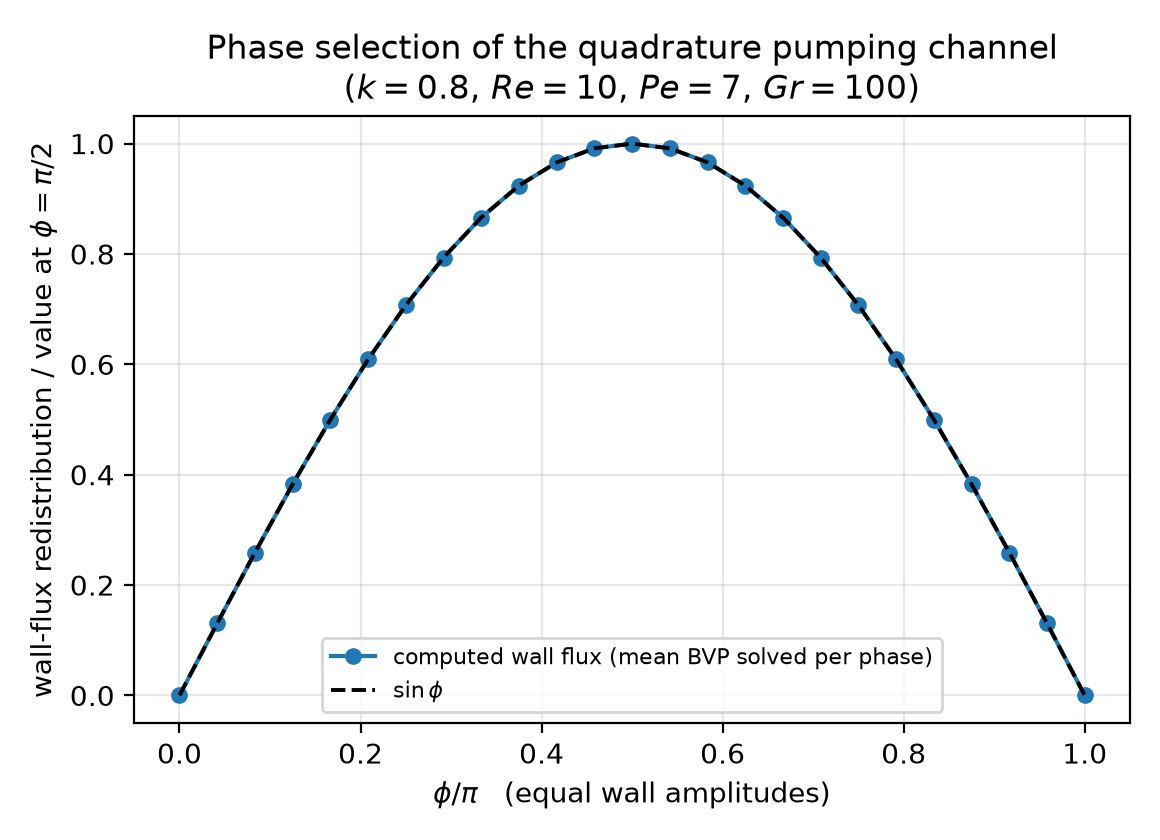
\includegraphics[width=0.62\textwidth]{campaign_v2_symmetry_selection/FIG_v2_07_sin_phi.png}
  \caption{Exact phase selection for equal wall amplitudes at
  $(k,\Pe,\Rey,\Pr,\Grr)=(0.8,7,10,0.7,100)$. Each marker is an independent
  calculation: the mixed forcing is re-assembled for that phase and the
  second-order mean thermal problem is re-solved, so the plot is not the
  analytic expression against itself. The computed normalized response lies on
  $\sin\phi$ (dashed) to within $2.4\times10^{-13}$; the response vanishes at
  the purely symmetric ($\phi=0$) and purely antisymmetric ($\phi=\pi$) phase
  relations.}
  \label{fig:sin_phi}
\end{figure}

\begin{figure}[htb]
  \centering
  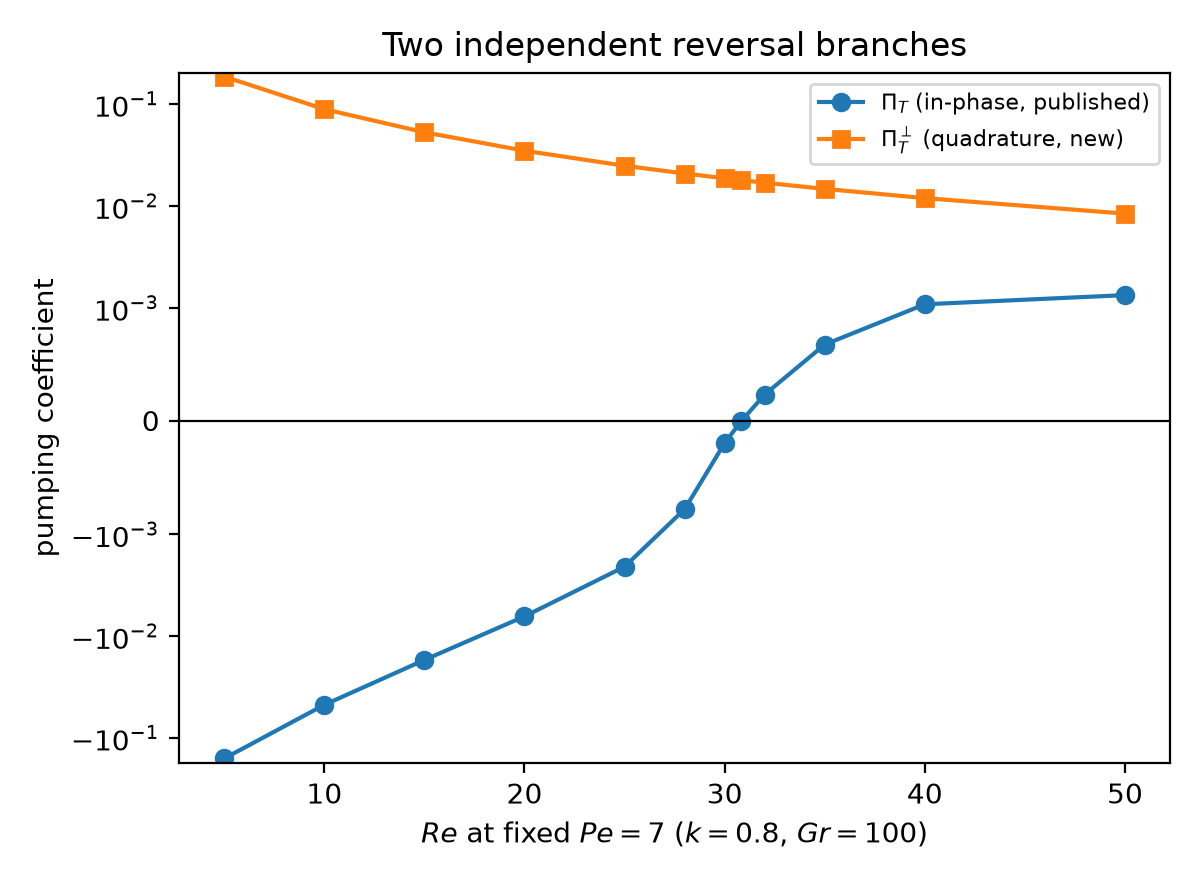
\includegraphics[width=0.66\textwidth]{campaign_v2_symmetry_selection/FIG_v2_06_two_branches.png}
  \caption{The two independent pumping coefficients versus Reynolds number at fixed
  $\Pe=7$, $k=0.8$ and $\Grr=100$. The in-phase coefficient $\PiT$ reverses at
  $\Rey_c=30.838$, while the quadrature coefficient $\PiT^{\perp}$ remains positive
  throughout the scanned interval and decays monotonically.}
  \label{fig:two_branches}
\end{figure}

%--------------------------------------------------------------
\section{Numerical Results and Validation}
\label{sec:results}
%--------------------------------------------------------------

\subsection{Numerical implementation and independent validation}

All first-order boundary-value problems are solved using the adaptive collocation algorithm
\texttt{solve\_bvp} from SciPy \cite{Virtanen2020}. The mixed second-order temperature field is obtained
from Eq.~\eqref{eq:theta_as_BVP}. The numerical audit is structured around independent consequences of the
analysis: BVP residuals and boundary conditions, reflection parity, forcing parity and integral identities,
wall-flux antisymmetry, the Green-function identity, collocation--shooting agreement, mesh sensitivity, and
the fixed-bulk-flow condition for the mean streaming correction. Supplementary Sec.~\ref{app:validation}
records the shooting formulation of both boundary-value problems, which is the independent reconstruction
behind the collocation--shooting agreement reported below.

At $(k,\Rey,\Pr,\Grr)=(2,10,0.7,100)$, the CPU reference calculation gives
\begin{equation}
  \Nu_{2,0}(+1)=1.9730398325\times10^{-3},\qquad
  \Nu_{2,0}(-1)=-1.9730398325\times10^{-3},
\end{equation}
and hence $\PiT=1.9730398325\times10^{-3}$. The independent integral representation agrees to within
$3.2\times10^{-13}$, and the quadrature cross-check is $O(10^{-11})$. The maximum parity residual is
below $7\times10^{-17}$ and the wall-flux antisymmetry residual below $9\times10^{-19}$. Independent
collocation--shooting field differences remain below $9\times10^{-12}$. The fixed-bulk-flow mean streaming
correction satisfies its integral constraint to $1.1\times10^{-16}$.

The reference result is also insensitive to the initial collocation mesh. Calculations with $N_0=101,201,401,801$
and a finer reference initialization differ from the reported value only in the last displayed digits.
These tests support the use of the adaptive collocation result as the authoritative CPU reference while the
shooting calculation supplies an independent field reconstruction.
Table~\ref{tab:validation_summary} collects the diagnostics of that audit.

\begin{table}[htb]
  \centering
  \caption{Representative numerical validation diagnostics for the reference case
  $(k,\Rey,\Pr,\Grr)=(2,10,0.7,100)$.}
  \label{tab:validation_summary}
  \begin{ruledtabular}
  \begin{tabular}{lc}
  Diagnostic & Maximum reported magnitude \\
  \hline
  First-order residuals & $1.5\times10^{-14}$ \\
  Thermal/velocity parity residuals & $6.8\times10^{-17}$ \\
  $\int\mathcal E_{as}\,dY$ & $4.3\times10^{-19}$ \\
  Wall-flux antisymmetry & $8.7\times10^{-19}$ \\
  Wall-vs-integral $\PiT$ discrepancy & $3.2\times10^{-13}$ \\
  Quadrature cross-check & $1.8\times10^{-11}$ \\
  Collocation--shooting difference & $8.6\times10^{-12}$ \\
  Zero-bulk-flux residual & $1.1\times10^{-16}$ \\
  \end{tabular}
  \end{ruledtabular}
\end{table}

\subsection{Grashof-number scaling}

A dedicated sweep at $(k,\Rey,\Pr)=(0.8,10,0.7)$ gives a free-intercept fit
\begin{equation}
  \PiT=(-4.7485\times10^{-4})\Grr-5.51\times10^{-16},
\end{equation}
with $R^2=1.000000$. The $\Grr=0$ calculation gives zero pumping to numerical precision, confirming
Eq.~\eqref{eq:PiT_Gr}; the sweep is plotted in Fig.~\ref{fig:Gr_sweep}.

\subsection{Finite-domain endpoint of the zero-crossing branch}
\label{subsec:critical_endpoint}

At fixed $\Rey=10$ and $\Grr=100$ the normalized response $A=\PiT/\Grr$
changes sign over the $(k,\Pe)$ domain, and the zero set
\begin{equation}
  \PiT(k^*,\Pe)=0
  \label{eq:zero_locus}
\end{equation}
defines an interior pumping-reversal branch wherever a sign change is present
within the admissible interval $0.02\le k\le10$. This branch terminates
because the interval is finite, not because of a bifurcation, and the
endpoint is therefore a property of the computational window.

Two calculations bracket that termination. Just below the endpoint the zero is
interior: at $\Pe=10.85$ the response changes sign once, at
\begin{equation}
  k^*=9.338218553141,
  \qquad
  \left|\PiT(k^*)\right|=1.92\times10^{-20}.
  \label{eq:interior_root_precise}
\end{equation}
At the endpoint itself the zero has reached the upper boundary,
\begin{equation}
  \boxed{
  \Pe_c=10.871940554611,\qquad k_c=10,
  }
  \label{eq:finite_domain_endpoint}
\end{equation}
where the boundary value $\PiT(10,\Pe_c)=-8.40\times10^{-15}$ is zero to the
resolution of the calculation. Just above the endpoint the positive branch is
gone: at $\Pe=10.9$ every sampled wavenumber gives a negative response and no
sign-change bracket exists, the largest (least negative) value being
$\PiT(10,10.9)=-1.4068443\times10^{-6}$.

\begin{figure}[htb]
  \centering
  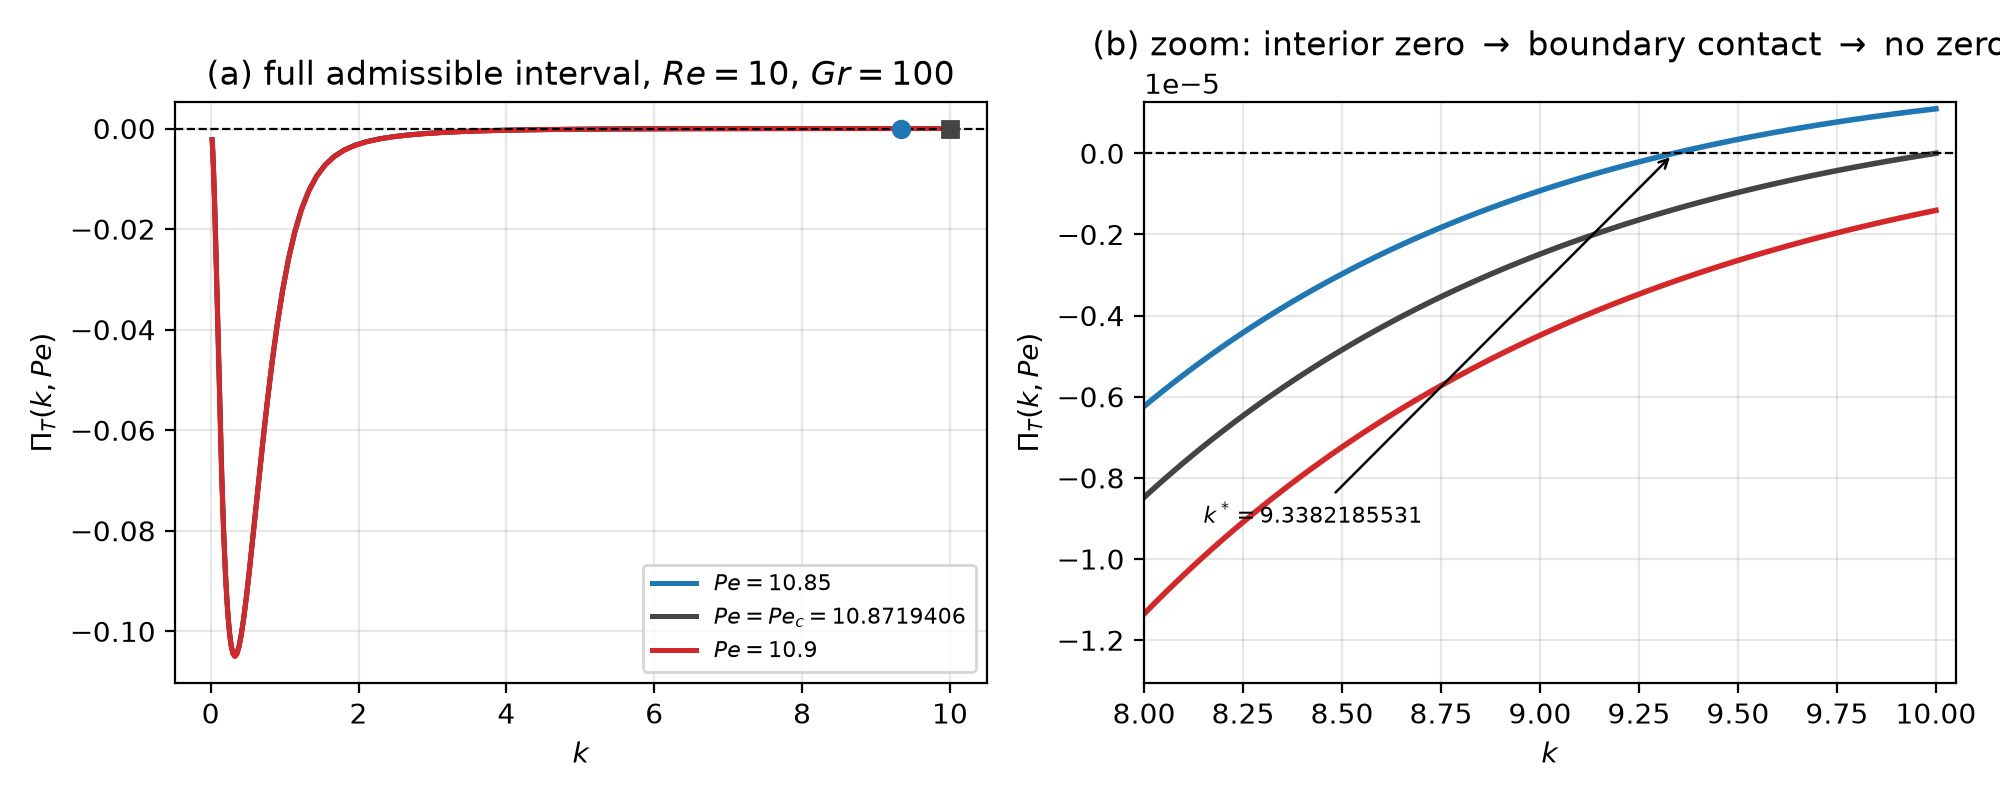
\includegraphics[width=0.82\textwidth]
  {campaign_v2_symmetry_selection/FIG_v2_09_Pe_c_endpoint.png}
  \caption{Termination of the interior zero-crossing branch at the finite
  upper wavenumber boundary ($\Rey=10$, $\Grr=100$). (a) Response
  $\PiT(k,\Pe)$ over the full admissible interval for the three retained
  calculations; the curves are visually indistinguishable at this scale,
  which is itself the point: the change of regime is a near-zero effect
  confined to $k\gtrsim8$. (b) High-wavenumber zoom. The interior zero at
  $k^*=9.3382185531$ for $\Pe=10.85$ migrates to the boundary $k=10$ at
  $\Pe=\Pe_c$ and disappears for $\Pe=10.9$.}
  \label{fig:endpoint}
\end{figure}

Figure~\ref{fig:endpoint} shows the three regimes in one view: interior zero,
boundary contact, and complete loss of positive response inside the window. The
endpoint is reached geometrically, when the zero set of $\PiT(k,\Pe)$ first touches
$k=k_{\max}=10$; it is not prescribed as an independent critical parameter. A dense local
check at that boundary confirms that the transition is transversal rather than a sampling
artefact: with $\delta=\Pe-\Pe_c$, the boundary value is
$\PiT(10,\Pe_c-\delta)=+5.00619\times10^{-8}$ and $+5.00641\times10^{-9}$ for
$\delta=10^{-3}$ and $10^{-4}$, and $\PiT(10,\Pe_c+\delta)=-5.00648\times10^{-9}$ and
$-5.00671\times10^{-8}$ for the same two offsets. The magnitudes are nearly antisymmetric
about $\Pe_c$, so the boundary value crosses zero with a finite local slope
$\partial\PiT/\partial\Pe\approx-5.01\times10^{-5}$ at $(k,\Pe)=(10,\Pe_c)$; the full
five-row ladder is in group A of the supplementary data package.

The endpoint must therefore be read strictly as a \emph{finite-domain dynamical endpoint}
of the observed zero-crossing branch for $(\Rey,\Grr)=(10,100)$ on $0.02\le k\le10$ --- not
a universal critical P\'eclet number, not an instability threshold. The survey supporting
this classification (173 wavenumbers per $\Pe$ for five $\Pe$ values, 865 first-order BVP
evaluations, plus the local $\Delta\Pe$ ladder quoted above) is archived as group
A of the supplementary data package, which records the raw grid, the refined roots, the
$\Delta\Pe$ ladder and the
run log of that survey; the two bracketing calculations
above are the ones used in the main text.

\subsection{Mean profile structure}

The second-order mean temperature correction and mean streaming velocity provide a complementary picture
of the redistribution mechanism. For one-sided asymmetric forcing ($\varepsilon_2=0$), the mixed mean
thermal correction is odd while the corresponding mean velocity correction reflects the accompanying momentum
redistribution under fixed bulk flow.

%--------------------------------------------------------------
\section{Independent Nonlinear DNS Validation}
\label{sec:dns_validation}
%--------------------------------------------------------------

The perturbation theory developed above is based on the assumption that the
wall-temperature modulation amplitude is sufficiently small for the asymptotic
expansion to remain valid through second order. Although the analytical results
are internally verified by the boundary-value and shooting formulations, an
independent nonlinear calculation is required to determine whether the
predicted pumping response persists in the fully coupled finite-amplitude
transport problem. We therefore perform a separate two-dimensional direct
numerical simulation (DNS) of the nonlinear Boussinesq equations.

The DNS does not use the first-order thermal or hydrodynamic modal solutions
as input. Instead, the fully nonlinear temperature and momentum equations are
integrated directly to a stationary state under the same periodic wall
forcing, with the wall heat-flux difference evaluated from the converged
temperature field. The DNS is consequently an independent test of the
perturbative mechanism rather than a second implementation of the same
boundary-value calculation. Four numbers from that campaign carry the argument
of Sec.~\ref{sec:outlook}: the parity cancellation measured at
$3.1\times10^{-18}$ in the wall-flux difference, the eight bracketed runs that
all return the predicted reversal sign, the Grashof ratio exact to
$3.7\times10^{-4}$, and the quadrature coefficient recovered to $1.38\%$.

Unless otherwise stated, the reference DNS configuration is
\begin{equation}
(k,\Pe,\Rey,\Pr,\Grr) = (0.8,7,10,0.7,100),
\end{equation}
with
\begin{equation}
\varepsilon_s=0.03,
\qquad
\varepsilon_a=0.005,
\end{equation}
so that
\begin{equation}
\varepsilon_1=0.035,
\qquad
\varepsilon_2=0.025.
\end{equation}
The nonlinear DNS is performed independently of the perturbative BVP
solver. The stationary state is accepted only after the residual of the
discretized evolution equations falls below the prescribed convergence
threshold and the wall-flux observables become stationary.

The DNS estimator mirrors the perturbative definition \eqref{eq:PiT_def} and
is formed from the cycle-averaged wall-normal wall heat fluxes $q_\pm$ alone.
Because $q_+-q_-$ is the fully nonlinear counterpart of
$\Nu_{2,0}(+1)-\Nu_{2,0}(-1)$, the coefficient recovered from the simulation is
\begin{equation}
  \PiT^{\mathrm{DNS}}
  \;=\;
  \frac{q_+-q_-}{2\varepsilon_a\varepsilon_s}.
  \label{eq:PiT_dns_estimator}
\end{equation}
For the reference configuration, $q_+-q_-=-1.40289979\times10^{-5}$ and
$2\varepsilon_a\varepsilon_s=3.0\times10^{-4}$, giving
$\PiT^{\mathrm{DNS}}=-4.6763\times10^{-2}$, the value quoted in
Table~\ref{tab:dns_validation_summary}. No first-order modal field enters the
estimator, which is what makes the comparison independent of the perturbative
solver.

\subsection{Amplitude convergence and recovery of the perturbative limit}
\label{subsec:dns_amplitude}

The first and most direct test concerns the asymptotic limit
$\varepsilon_a\rightarrow0$. Because the leading pumping contribution is
proportional to the mixed product $\varepsilon_a\varepsilon_s$, the
normalized coefficient extracted from the nonlinear DNS should approach a
finite limit as the asymmetry amplitude decreases. We therefore performed a
sequence of DNS calculations with decreasing $\varepsilon_a$ while keeping
$\varepsilon_s=0.03$ fixed.

The resulting values of the nonlinear pumping coefficient are
\begin{equation}
\begin{array}{c|c}
\varepsilon_a & \PiT^{\mathrm{DNS}}\\
\hline
0.0150 & -4.67629365\times10^{-2}\\
0.0100 & -4.67631801\times10^{-2}\\
0.0075 & -4.67632654\times10^{-2}\\
0.0050 & -4.67633263\times10^{-2}
\end{array}
\end{equation}
and the extrapolation to $\varepsilon_a\rightarrow0$ gives
\begin{equation}
\PiT^{\mathrm{DNS},\,\varepsilon_a\rightarrow0}
\simeq -4.6763\times10^{-2}.
\end{equation}
The perturbative prediction for the same reference state is
\begin{equation}
\PiT^{(2)} = -4.7485\times10^{-2},
\end{equation}
corresponding to a relative difference of approximately
$1.52\%$.

This agreement is significant for two reasons. First, the DNS solves the
nonlinear problem at finite wall-modulation amplitude rather than the
asymptotically truncated equations. Second, the observed convergence of
$\PiT^{\mathrm{DNS}}$ as $\varepsilon_a$ decreases demonstrates that the nonlinear
solution approaches a finite coefficient consistent with the second-order
theory. The result therefore supports the interpretation of $\PiT$ as the
leading nonlinear transport coefficient associated with the
symmetric--antisymmetric interaction (Fig.~\ref{fig:dns_amplitude}).

\subsection{Spatial and temporal convergence}
\label{subsec:dns_convergence}

The numerical reliability of the DNS observable is assessed independently
through grid and time-step refinement. For the spatial study, the calculation
was performed on progressively refined meshes
$48\times37$, $64\times49$, $80\times61$, and $96\times73$. The corresponding
pumping coefficients are
\begin{equation}
\begin{array}{c|c|c}
N_x\times N_y & \PiT^{\mathrm{DNS}} &
\text{relative difference from finest grid}\\
\hline
48\times37 & -4.65557743\times10^{-2} & 1.10\%\\
64\times49 & -4.67633263\times10^{-2} & 0.66\%\\
80\times61 & -4.69453055\times10^{-2} & 0.27\%\\
96\times73 & -4.70739712\times10^{-2} & 0
\end{array}
\end{equation}
where the finest mesh is used only as the numerical reference for the
convergence study. The monotonic variation toward the finest-grid solution
indicates that the wall-flux observable is spatially resolved rather than
being controlled by under-resolution of the transverse boundary layers
(Fig.~\ref{fig:dns_spatial}).

The temporal convergence study gives
\begin{equation}
\begin{array}{c|c|c}
\Delta t & \PiT^{\mathrm{DNS}} &
\text{relative difference from smallest }\Delta t\\
\hline
3.0\times10^{-3}
& -4.67632768\times10^{-2}
& 1.75\times10^{-6}\\
2.0\times10^{-3}
& -4.67633588\times10^{-2}
& 1.38\times10^{-9}\\
1.5\times10^{-3}
& -4.67633263\times10^{-2}
& 6.95\times10^{-7}\\
1.0\times10^{-3}
& -4.67633588\times10^{-2}
& 0
\end{array}
\end{equation}
The extremely small change in $\PiT$ over this sequence shows that the reported
pumping coefficient is not controlled by the chosen temporal discretization
(Fig.~\ref{fig:dns_timestep}).

The convergence histories provide an additional stationarity check. At the
reference resolution, the final evolution residual is
\begin{equation}
\mathcal{R}_{\mathrm{DNS}}\lesssim 7\times10^{-9},
\end{equation}
while the global wall-flux balance satisfies
\begin{equation}
q_+ + q_-
\simeq -1.9\times10^{-7}.
\end{equation}
These values show that the reported $\PiT$ is extracted from a genuinely
converged stationary state rather than from an arbitrary finite-time snapshot.

\subsection{Independent verification of the Grashof-number scaling}
\label{subsec:dns_gr}

The analytical formulation predicts that the first-order hydrodynamic response
is proportional to $\Grr$ and therefore that, at fixed $(k,\Rey,\Pr)$,
\begin{equation}
\PiT=\Grr A(k,\Rey,\Pr).
\end{equation}
This prediction is tested directly with fully nonlinear DNS by varying
$\Grr$ from zero to $200$ while retaining the same geometry, Reynolds number,
and thermal parameters.

The DNS gives a practically linear dependence over the investigated range,
with a coefficient of determination indistinguishable from unity at the
reported numerical precision. In addition, the zero-buoyancy simulation gives
\begin{equation}
\PiT(\Grr=0)
\simeq -1.1\times10^{-14},
\end{equation}
which is numerically zero (Fig.~\ref{fig:dns_gr}).

This result is particularly useful because it validates a structural
prediction that is independent of the spatial-parity proof. The symmetry
theorem determines the admissible relation between the two wall-flux
corrections, while the present DNS confirms independently that the strength
of this redistribution is controlled linearly by the buoyancy amplitude at
leading order.

\subsection{Reynolds-number control at fixed P\'eclet number}
\label{subsec:dns_re}

A central consequence of the governing equations is that $\Pe$ cannot in
general be treated as the sole control parameter for the pumping coefficient.
The thermal modal problem depends on $\Pe=\Rey\,\Pr$, but the hydrodynamic response
retains explicit dependence on $\Rey$. The fully nonlinear DNS provides an
independent physical test of this distinction.

We therefore keep
\begin{equation}
\Pe=7,\qquad \Grr=100,\qquad k=0.8
\end{equation}
fixed and vary $\Rey$, adjusting the Prandtl number according to
\begin{equation}
\Pr=\frac{\Pe}{\Rey}.
\end{equation}
The normalized pumping response obtained from DNS is
\begin{equation}
\begin{array}{c|c|c|c}
\Rey & \Pr & A_{\mathrm{DNS}}=\PiT/\Grr & \operatorname{sign}(A_{\mathrm{DNS}})\\
\hline
5
& 1.4000
& -1.5878\times10^{-3}
& -\\
10
& 0.7000
& -4.6763\times10^{-4}
& -\\
20
& 0.3500
& -5.9977\times10^{-5}
& -\\
30
& 0.2333
& +7.5042\times10^{-7}
& +\\
35
& 0.2000
& +8.9842\times10^{-6}
& +
\end{array}
\end{equation}

The independent DNS therefore reproduces a clear reversal of the pumping
direction. The response is negative at $\Rey=20$ but has become positive by
$\Rey=30$, demonstrating directly that changing the hydrodynamic Reynolds
number while preserving the same $\Pe$ can reverse the direction of nonlinear
thermal pumping (Fig.~\ref{fig:dns_re}).

The corresponding perturbative values of $A$ at $\Rey=5$, $10$, $20$, and $35$ are
$-1.5951\times10^{-3}$, $-4.7485\times10^{-4}$,
$-6.4279\times10^{-5}$, and $+6.7452\times10^{-6}$, respectively. The
quantitative agreement is strongest at the lower and intermediate Reynolds
numbers, with relative differences of $0.46\%$, $1.52\%$, and $6.69\%$ for
$\Rey=5$, $10$, and $20$. At $\Rey=35$, the relative difference increases to
$33.19\%$; however, both the DNS and perturbative responses are very small in
absolute magnitude and have the same positive sign. The discrepancy therefore
reflects the sensitivity of a relative error metric near a zero crossing rather
than a disagreement in the qualitative pumping mechanism. Near the reversal,
the sign of the response is therefore a more robust diagnostic than a relative
error normalized by a quantity approaching zero.

The principal physical result of this sweep is thus not the absolute value at
$\Rey=35$, but the independently confirmed reversal of the pumping direction.
This observation supports the analytical conclusion that $A$ is, in general,
a function of $(k,\Rey,\Pr)$ and cannot be reduced universally to a function
of $(k,\Pe)$ alone; Table~\ref{tab:dns_re_sweep} lists the sweep.

\subsection{Independent verification of reflection symmetry and conservation}
\label{subsec:dns_symmetry}

The exact parity theorem predicts two particularly strong properties that can
be tested without comparing the DNS with any perturbative amplitude:
(i) reflection of the upper and lower wall amplitudes must reverse the
direction of the wall-flux redistribution, and (ii) perfectly symmetric
wall forcing must suppress the directional pumping observable.

For the asymmetric reference case, the DNS gives
\begin{equation}
q_+-q_- = -1.40289979\times10^{-5},
\end{equation}
whereas after interchanging the upper and lower wall amplitudes,
\begin{equation}
q_+-q_- = +1.40289979\times10^{-5}.
\end{equation}
The corresponding reflection residual is
\begin{equation}
\left|
D_{\rm reflected}+D_{\rm baseline}
\right| = 3.18\times10^{-17}.
\end{equation}

For perfectly symmetric wall forcing, the DNS gives
\begin{equation}
q_+-q_- = 8.13\times10^{-18},
\end{equation}
which is indistinguishable from zero at the resolution of the simulation
(Fig.~\ref{fig:dns_symmetry}).

\begin{figure}[htb]
\centering
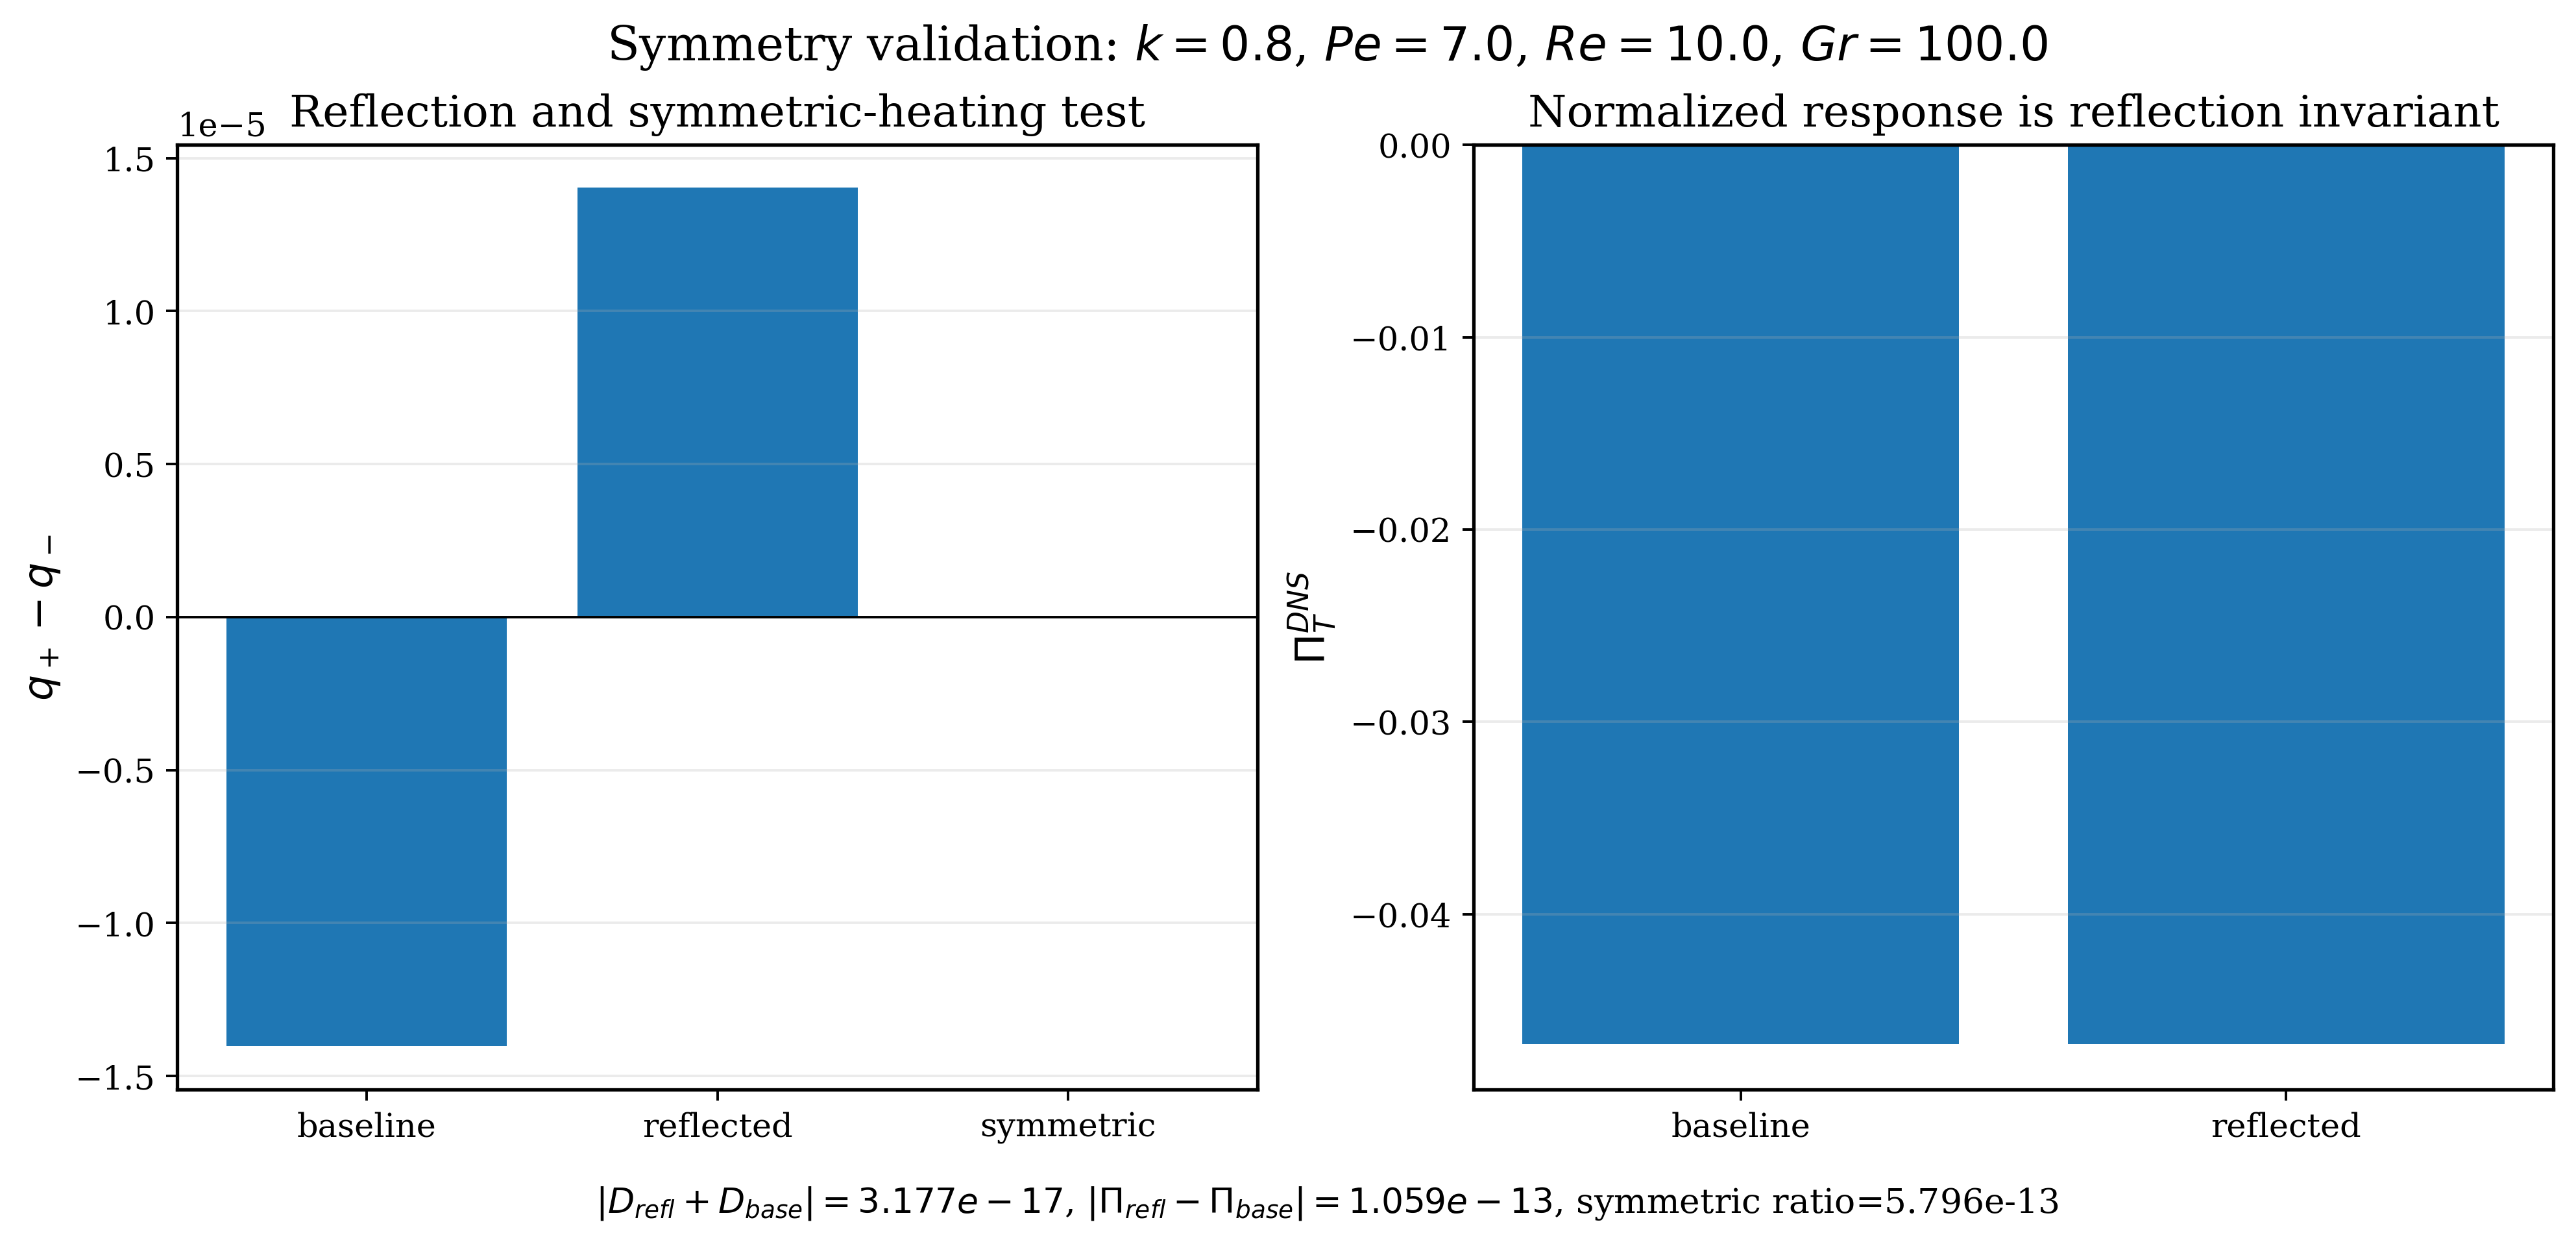
\includegraphics[width=0.78\textwidth]
{FIG06_dns_symmetry_conservation.png}
\caption{
Independent DNS verification of reflection symmetry and wall-flux
conservation. Interchanging the upper and lower thermal forcing reverses the
sign of the wall-flux difference, whereas perfectly symmetric forcing
suppresses the directional redistribution. The measured symmetry residuals
are at or below $10^{-13}$, with the direct flux-reflection residual reaching
$3.18\times10^{-17}$.
}
\label{fig:dns_symmetry}
\end{figure}

The DNS therefore reproduces the structural symmetry law without explicitly
enforcing the analytical parity relations. This is an important distinction:
the perturbative derivation proves the selection rule analytically, whereas
The nonlinear DNS independently recovers the same reflection-induced reversal
of the wall-flux difference and the suppression of directional redistribution
under symmetric forcing. Thus, the symmetry-selected structure identified
analytically is also observed in the fully coupled nonlinear calculation at
finite modulation amplitude.

\subsection{Consolidated validation}
\label{subsec:dns_summary}

Figure~\ref{fig:dns_summary} summarizes the independent numerical evidence.
The combination of amplitude extrapolation, spatial refinement, time-step
refinement, Grashof-number scaling, Reynolds-number sweeps, reflection tests,
and wall-flux conservation provides validation at three complementary levels.

First, the amplitude and resolution studies establish numerical convergence of
the nonlinear observable. Second, the $\Grr$ and symmetry studies verify the
structural consequences of the analytical framework. Third, the fixed-$\Pe$
Reynolds sweep provides a genuinely physical result that is not contained in
the parity proof alone: the direction of nonlinear pumping can be selected by
the hydrodynamic Reynolds number while the thermal P\'eclet number is unchanged.

\begin{figure}[htb]
\centering
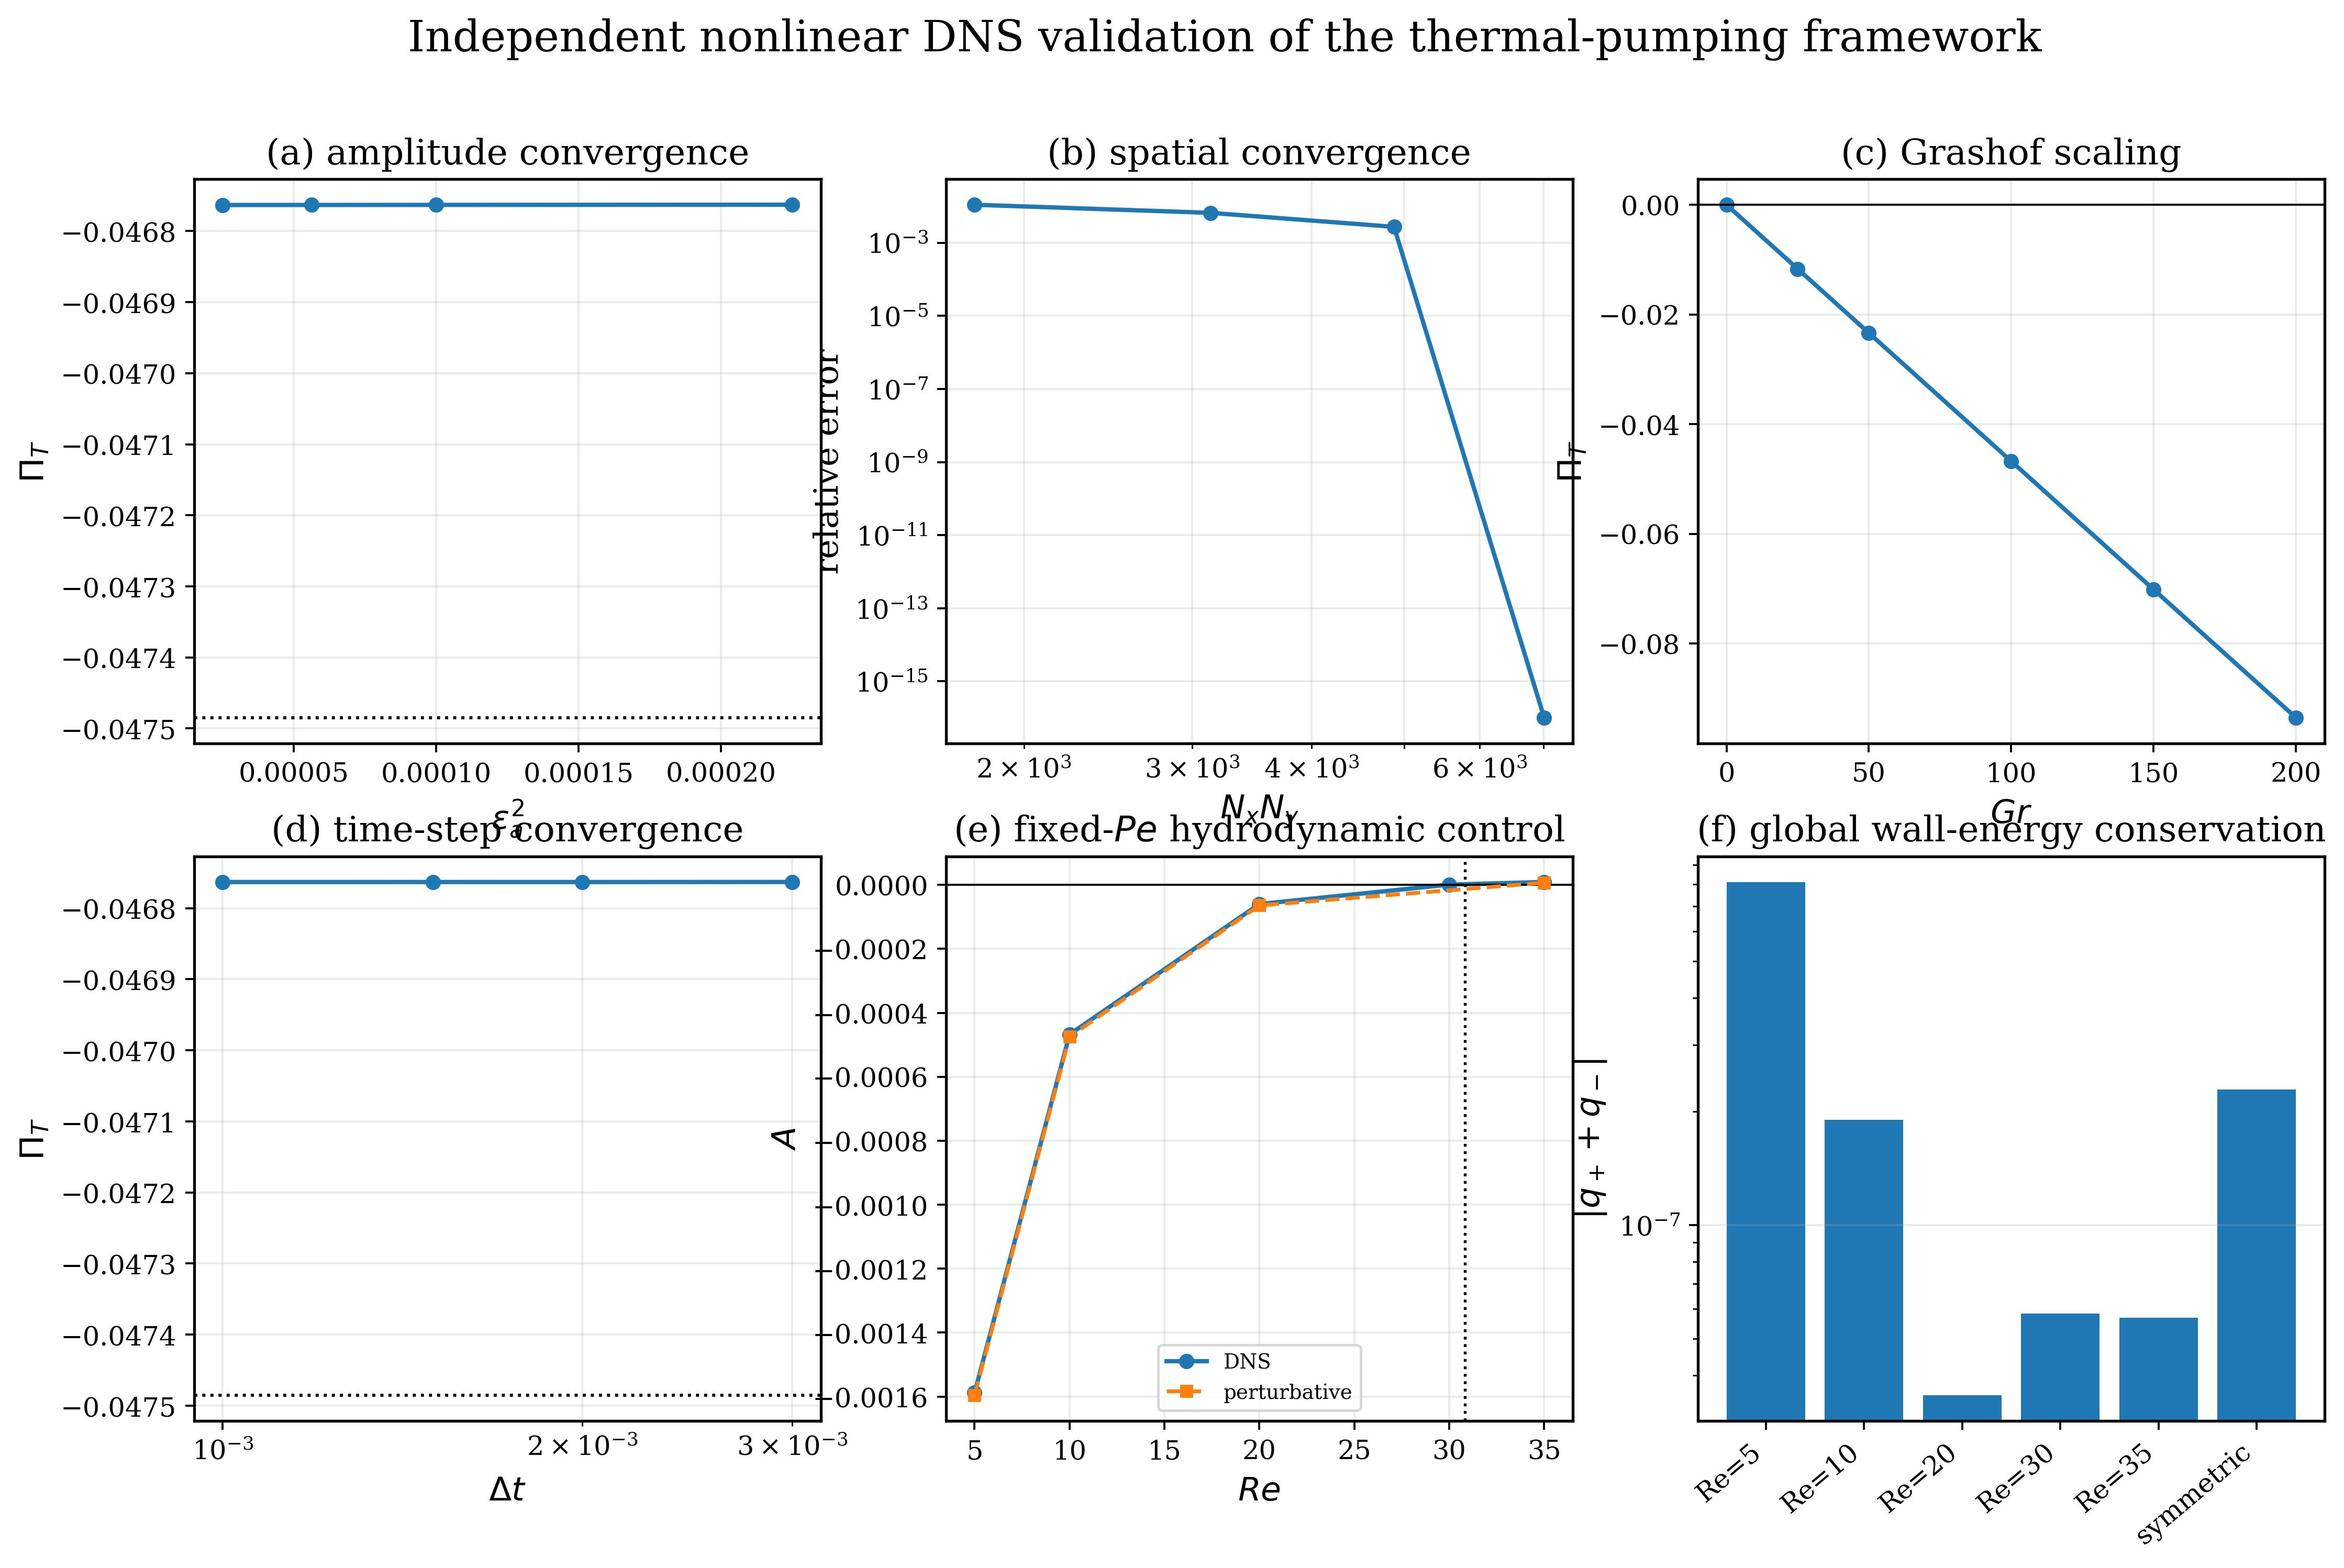
\includegraphics[width=0.96\textwidth]
{FIG07_dns_validation_summary.png}
\caption{
Consolidated summary of the independent nonlinear DNS validation campaign.
The seven diagnostic panels combine amplitude extrapolation, spatial and
temporal convergence, Grashof-number scaling, fixed-$\Pe$ Reynolds dependence,
and wall-flux conservation. Together they show that the perturbative
thermal-pumping framework is recovered by an independent nonlinear
computation and that the Reynolds number remains an active control parameter
for the direction of the pumping response.
}
\label{fig:dns_summary}
\end{figure}

For convenience, the principal validation results are collected in
Fig.~\ref{fig:dns_summary} and Table~\ref{tab:dns_validation_summary}. The spatial and temporal entries are
reported as differences from the finest calculation in the corresponding
convergence sequence; they therefore do not represent formal discretization
error bounds.

\begin{table}[htb]
\centering
\caption{
Summary of the independent nonlinear DNS validation campaign. Spatial and
temporal convergence values are measured relative to the finest calculation
in each sequence. Reflection and symmetric-forcing residuals are absolute
numerical residuals.
}
\label{tab:dns_validation_summary}
\begin{ruledtabular}
\footnotesize
\setlength{\tabcolsep}{5pt}
\begin{tabular}{@{\hspace{4pt}}lccc@{\hspace{4pt}}}
Test & DNS result & Reference or criterion & Assessment \\
\hline
Amplitude extrapolation
& $-4.6763\times10^{-2}$
& $-4.7485\times10^{-2}$
& $1.52\%$ difference \\
Spatial convergence
& $<1.10\%$
& finest-grid limit
& converged \\
Time-step convergence
& $<1.8\times10^{-6}$
& smallest-$\Delta t$ limit
& converged \\
$\Grr$ scaling
& $R^2\simeq1$
& linearity
& confirmed \\
$\Grr=0$
& $\left|\PiT\right|\simeq1.1\times10^{-14}$
& $0$
& confirmed \\
Reflection flux residual
& $3.18\times10^{-17}$
& $0$
& confirmed \\
Reflection $\PiT$ residual
& $1.06\times10^{-13}$
& $0$
& confirmed \\
Symmetric forcing residual
& $5.80\times10^{-13}$
& $0$
& confirmed \\
\end{tabular}
\end{ruledtabular}
\end{table}

Taken together, these calculations provide an independent nonlinear
verification of the main analytical conclusions without requiring the DNS to
reproduce every perturbative coefficient to arbitrary relative accuracy near
a zero crossing. The strongest quantitative agreement occurs away from the
reversal region, whereas the vicinity of the reversal is characterized by
excellent agreement in the sign and by enhanced sensitivity of the relative
error to small absolute differences. This behavior is physically consistent
with the interpretation of the pumping response as the result of competing
thermal--hydrodynamic pathways.

\subsection{Physical implication of the nonlinear DNS validation}
\label{subsec:dns_physical_implication}

The DNS results strengthen the physical interpretation of the pumping mechanism
by demonstrating that the symmetry-selected wall-flux redistribution is not an
artifact of the perturbative truncation. The exact reflection properties survive
in the fully nonlinear equations, while the magnitude and direction of the
response remain dynamically selectable. In particular, the fixed-$\Pe$
Reynolds sweep shows that the thermal field and hydrodynamic mediator should
not be viewed as a single reduced transport process: $\Pe$ controls the thermal
competition between advection and diffusion, whereas $\Rey$ independently
modulates the buoyancy-induced velocity field that transports the asymmetric
thermal mode. The observed reversal of $\PiT$ therefore provides a physical
signature of competing hydrodynamic pathways underlying the symmetry-selected
thermal redistribution.

%--------------------------------------------------------------
\section{Systematic Mapping of the Reynolds-Number Reversal}
\label{sec:reversal}
%--------------------------------------------------------------

The reversal reported above is obtained from fully nonlinear DNS at a single
wavenumber, and a single point cannot distinguish a law from an accident. We therefore
map the reversal locus $\Rey_c(k)$ with the authoritative perturbative solver over
seven wavenumbers at fixed $\Pe=7$ and $\Grr=100$, with $\Pr=\Pe/\Rey$, scanning
$\Rey\in\{5,10,15,20,25,30,35,40\}$ and refining each sign change by Brent
iteration. Because the two longest-wavelength crossings fall outside that
interval, the scan was extended for $k=0.4$ and $k=0.6$ up to $\Rey=120$.
Section~\ref{sec:outlook} confirms this locus nonlinearly: DNS run on both sides
of the crossing at four of the seven wavenumbers returns the predicted sign in
every case.
The complete grid and the seven refined crossings are archived with this paper as
group B of the supplementary data package.

\begin{table}[htb]
  \centering
  \caption{Reversal Reynolds number at fixed $\Pe=7$ and $\Grr=100$. The five
  entries with $\Rey_c\le40$ are bracketed inside the primary scan; the two
  longest-wavelength crossings lie beyond $\Rey=40$ and were bracketed on the
  extended interval. The reversal is therefore resolved at every wavenumber
  sampled. The $k=0.8$ value reproduces the independent determination from the
  DNS-based sweep, $\Rey_c=30.838496518$, to nine significant digits.}
  \label{tab:Rec_k}
  \begin{ruledtabular}
  \footnotesize
  \setlength{\tabcolsep}{4pt}
  \begin{tabular}{@{\hspace{3pt}}c|rrrrrrr@{\hspace{3pt}}}
  $k$              & 0.4 & 0.6 & 0.8 & 1.0 & 1.2 & 1.5 & 2.0 \\ \hline
  $\Rey_c(k)$      & 79.080214 & 51.252439 & 30.838497 & 20.487029 & 15.089038 & 11.069430 & 8.541316 \\
  \end{tabular}
  \end{ruledtabular}
\end{table}

Two facts follow. First, the reversal is systematic rather than isolated: it
occurs at every one of the seven wavenumbers sampled and its location moves
monotonically to lower $\Rey$ as $k$ increases, from $\Rey_c=79.08$ at $k=0.4$
to $\Rey_c=8.54$ at $k=2.0$. Over the seven resolved crossings the empirical
description $\Rey_c\approx21.50\,k^{-1.47}$ holds with a maximum relative
deviation of $11.0\%$; restricting the fit to the five crossings of the primary
$\Rey\le40$ window gives $\Rey_c\approx20.91\,k^{-1.41}$ with a maximum
deviation of $7.7\%$, so the two extra points do not follow the same power law
as closely as the interior ones. We report both as fits, not as derived
scalings, because no exponent has been obtained analytically. Second, the
reversal boundary of the $(k,\Rey)$ plane is not a finite wall at
$\Rey\approx40$: it recedes toward large $\Rey$ as $k$ decreases, and at
$\Grr=100$ the longest waves reverse only in the low-$\Pr$ corner of the
$(\Rey,\Pr)$ plane ($\Rey=79.08$ and $\Pr=0.089$ at $k=0.4$).
Fig.~\ref{fig:Rec_kartsch} draws the seven responses whose crossings define that boundary, and
Fig.~\ref{fig:Rec_locus} the refined locus with its power-law fit.

\begin{figure}[htb]
  \centering
  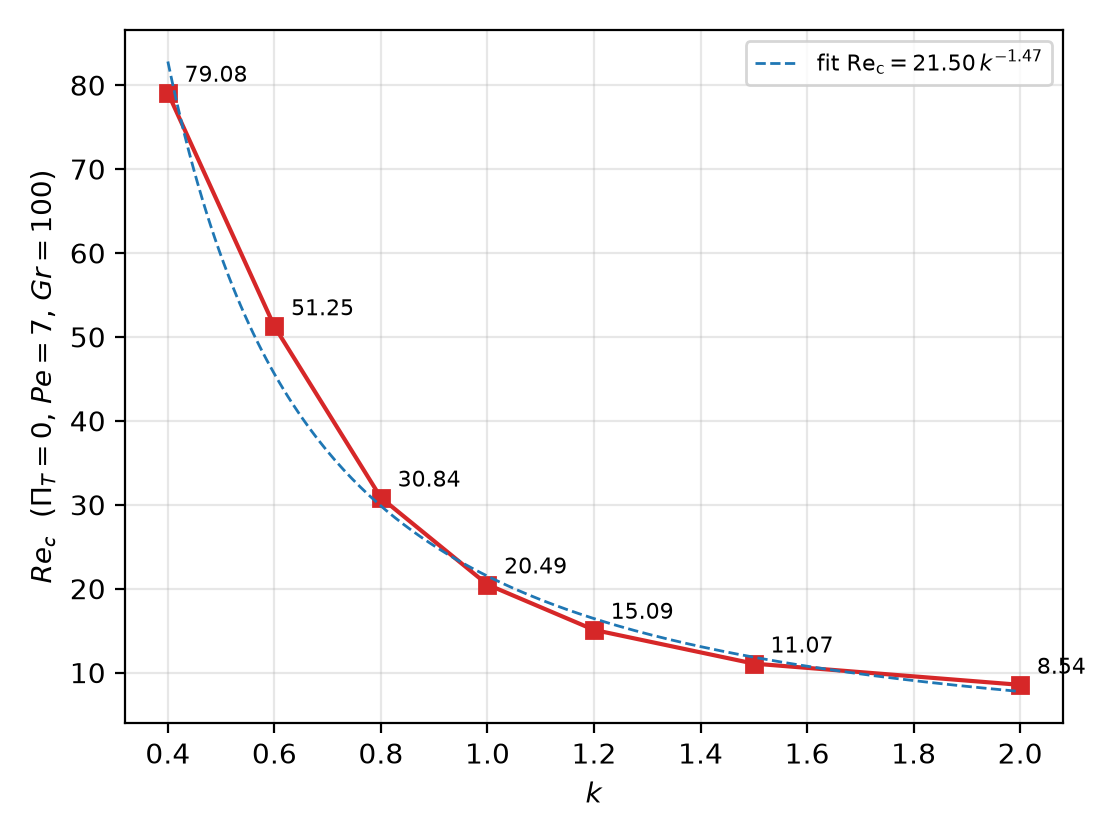
\includegraphics[width=0.55\textwidth]{campaign_v2_symmetry_selection/FIG_v2_02_Re_c_vs_k.png}
  \caption{Refined reversal locus $\Rey_c(k)$ at $\Pe=7$, $\Grr=100$ (Brent
  iteration on the perturbative solver), resolved at all seven sampled
  wavenumbers; the dashed line is the seven-point power-law fit
  $\Rey_c=21.50\,k^{-1.47}$. The $k=0.8$ point coincides with the value
  previously obtained from the fixed-$\Pe$ critical-Reynolds analysis.}
  \label{fig:Rec_locus}
\end{figure}

\subsection{Grashof-independence of the reversal: direct test of Corollary~\ref{cor:Gr_independence}}
\label{subsec:Gr_test}

Corollary~\ref{cor:Gr_independence} predicts that the reversal location does not move
when the buoyancy amplitude is changed. This is tested at $k=0.8$, $\Pe=7$ by locating
$\Rey_c$ independently for four Grashof numbers.

The invariance is exact to the convergence tolerance of the solver, which is the
strongest form of confirmation available for a structural prediction: the reversal
point is a property of $A(k,\Rey,\Pr)$ and not of the buoyancy amplitude; the four branches are
overlaid in Fig.~\ref{fig:Gr_invariance}. The same test
applied to the quadrature coefficient $\PiT^{\perp}$ gives an invariant
$\PiT^{\perp}/\Grr$ to $3.7\times10^{-13}$ over $\Grr=25$--$400$.

The same statement can be tested without the perturbative solver. A $2\times2$
DNS matrix at $k=0.8$ and $\Pe=7$ pairs $\Grr=50$ with $\Grr=200$ at two Reynolds
numbers straddling $\Rey_c$, one below and one above. The measured Grashof ratios
of $q_+-q_-$ are $4.0003$ at $\Rey=20$ and $4.0015$ at $\Rey=50$, against the exact
$4$ required by Corollary~\ref{cor:Gr_independence}: a worst-case relative error of
$3.7\times10^{-4}$, while the response amplitude itself changes by a factor of
four. The sign is unchanged within each pair---negative at $\Rey=20$, positive at
$\Rey=50$---so the reversal does not move when the buoyancy amplitude is quadrupled
in the fully nonlinear regime. The offset between DNS and the perturbative
coefficient is itself proportional to $\Grr$ (the two deviations of a pair differ
by $3.996$ and $4.015$), which is why it rescales the response without displacing
its zero: the relative error of $A=\PiT/\Grr$ is the same at both Grashof numbers,
$6.69\%$ at $\Rey=20$ and $10.7\%$ at $\Rey=50$. The checkpoint record of the
four runs, archived as group C of the data package, reduces to Table~\ref{tab:Gr_dns} and to
Fig.~\ref{fig:dns_grpair}, which draws the same statement as a single branch:
the reduced coefficient $A=\PiT/\Grr$ measured at the two Grashof numbers falls on
one curve, and that curve crosses zero at the perturbative $\Rey_c$. The four runs
cost $491$\,s in total, with residuals below $1.0\times10^{-8}$.

\begin{table}[htb]
  \centering
  \caption{Nonlinear test of Corollary~\ref{cor:Gr_independence} at $k=0.8$,
  $\Pe=7$, $\varepsilon_s=0.030$, $\varepsilon_a=0.005$ and $\phi=0$, with
  $\Pr=\Pe/\Rey$. Exact linearity in $\Grr$ forces the ratio of the two measured
  flux differences at each $\Rey$ to equal $200/50=4$; the ratios are $4.0003$
  and $4.0015$. The margin column is $|\PiT|$ in units of the deviation model
  $\delta_\Pi$; the raw record is archived as group C of the data package.}
  \label{tab:Gr_dns}
  \begin{ruledtabular}
  \begin{tabular}{rrrrrr}
  $\Rey$ & $\Grr$ & $\Pr$ & $q_+-q_-$ predicted & measured & margin \\ \hline
  20 & 50   & 0.3500 & $-9.641824\times10^{-7}$ & $-8.996526\times10^{-7}$ & 11.9 \\
  20 & 200  & 0.3500 & $-3.856730\times10^{-6}$ & $-3.598839\times10^{-6}$ & 47.4 \\
  50 & 50   & 0.1400 & $+1.994872\times10^{-7}$ & $+2.207512\times10^{-7}$ & 2.5 \\
  50 & 200  & 0.1400 & $+7.979489\times10^{-7}$ & $+8.833327\times10^{-7}$ & 9.8 \\
  \end{tabular}
  \end{ruledtabular}
\end{table}

\begin{figure}[htb]
  \centering
  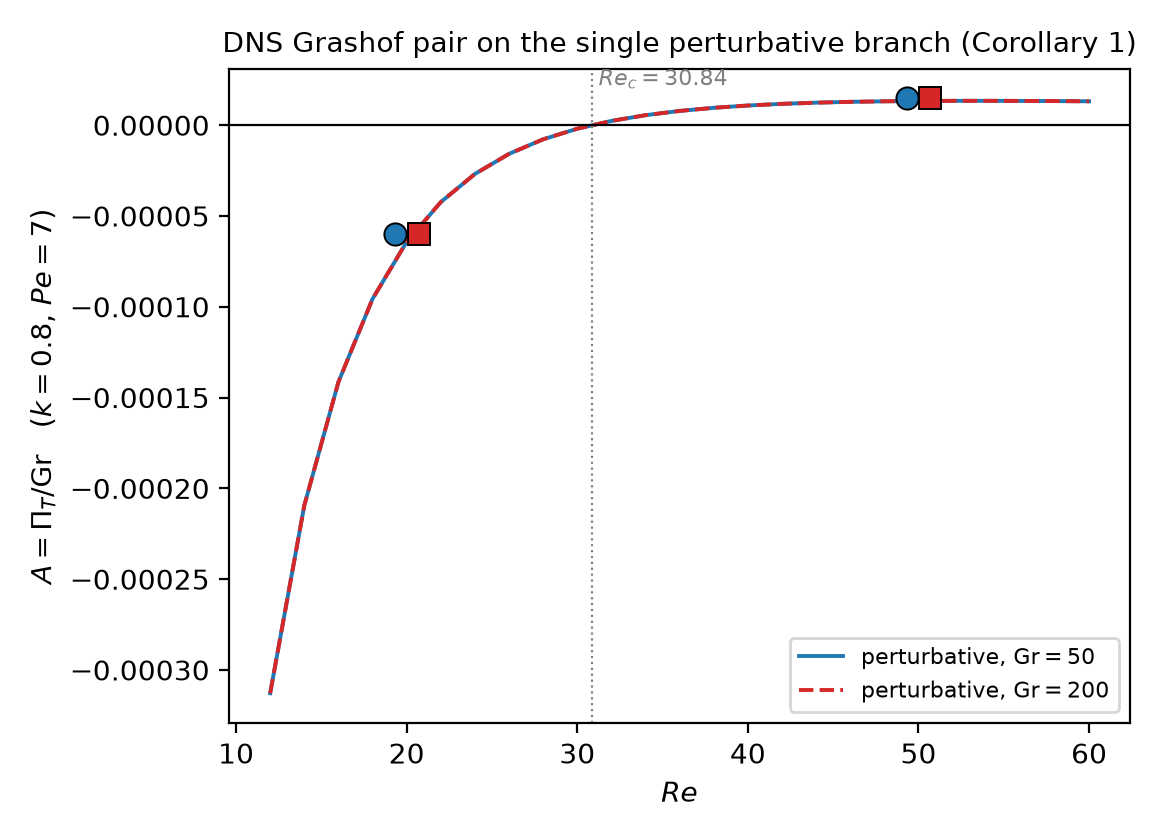
\includegraphics[width=0.62\textwidth]
  {campaign_v2_symmetry_selection/FIG_v2_11_dns_grpair.png}
  \caption{Nonlinear reading of Corollary~\ref{cor:Gr_independence}: the reduced
  coefficient $A=\PiT/\Grr$ versus $\Rey$ at $k=0.8$, $\Pe=7$. The two
  perturbative branches, $\Grr=50$ (solid) and $\Grr=200$ (dashed), are computed
  independently and separate by at most $1.1\times10^{-10}$ in relative terms,
  which is the $\Grr$-independence of $A$ and of its zero $\Rey_c=30.84$. The
  markers are the four DNS measurements of Table~\ref{tab:Gr_dns}: circles at
  $\Grr=50$, squares at $\Grr=200$, offset by $\pm0.7$ in $\Rey$ for legibility.
  Within each pair the two DNS values of $A$ agree to $6.3\times10^{-5}$
  ($\Rey=20$) and $3.7\times10^{-4}$ ($\Rey=50$), so the nonlinear response
  falls on the same single branch at both buoyancy amplitudes; the branch itself
  is approached to $6.7\%$ and $10.7\%$, the deviation analysed in
  Sec.~\ref{subsec:error_model}. The measured values and the reduced data of the
  two branches are archived as group C of the data package.}
  \label{fig:dns_grpair}
\end{figure}

The design is not accidental: candidate Reynolds numbers closer to the crossing
were rejected before integration by the resolvability gate of
Sec.~\ref{subsec:error_model}, which requires the predicted signal to exceed
the deviation floor by more than a
factor of two. The pair $\Rey=32$ has margins $0.43$ and $1.72$ and the pair
$\Rey=40$ has $1.99$ and $7.98$, so in both cases at least one member cannot
test a sign; the accepted pair keeps margins between $2.5$ and $47.4$ on both
sides of $\Rey_c$.

The residual departures of the two measured ratios from exactly four---$0.1\%$
and $0.4\%$---are not interpreted. A Richardson-type correction
$\Grr/\Rey^{2}$ would predict the larger departure at the smaller Reynolds
number, since $\Grr/\Rey^{2}=0.50$ for $(\Grr,\Rey)=(200,20)$ against $0.08$ for $(200,50)$,
whereas the observed ordering is the reverse. The ratios are therefore reported
as consistent with exact Grashof linearity at the tolerance the runs reach, and
the structural claim rests on the proportionality of the \emph{discrepancy}
together with the unchanged sign, not on the fourth decimal of the ratio.

%--------------------------------------------------------------
\section{Physical Interpretation and Discussion}
\label{sec:discussion}
%--------------------------------------------------------------

\subsection{Quantitative phase analysis of the reversal}
\label{sec:phase_analysis}

The reversal must be explained, not merely reported. Because the mean thermal problem
and the wall-flux functional $\mathcal L[\cdot]$ are linear, the four terms of the mixed
forcing \eqref{eq:kernels} contribute additively to $\PiT$:
\begin{equation}
  \PiT=\mathcal L\!\big[\langle V^{(a)}\partial_Y\Theta^{(s)}\rangle\big]
       +\mathcal L\!\big[\langle U^{(a)}\partial_X\Theta^{(s)}\rangle\big]
       +\mathcal L\!\big[\langle V^{(s)}\partial_Y\Theta^{(a)}\rangle\big]
       +\mathcal L\!\big[\langle U^{(s)}\partial_X\Theta^{(a)}\rangle\big],
  \label{eq:term_decomp}
\end{equation}
where $\langle\cdot\rangle$ denotes streamwise averaging and each term is evaluated with
the other mode at unit amplitude. Eq.~\eqref{eq:term_decomp} is an identity, not a
model: evaluating the four functionals separately reproduces the full $\PiT$ with a
maximum absolute deviation of $1.4\times10^{-14}$ over the whole $\Rey$ scan
(the relative deviation reaches $1.6\times10^{-5}$ only at $\Rey=\Rey_c$, where
$\PiT$ itself vanishes; Table~\ref{tab:term_balance}).

Three conclusions follow, and one common expectation is disproved.

\begin{enumerate}
  \item \textbf{The reversal is a magnitude race, not a phase flip.} The ratio of the
  two dominant contributions,
  $\big|\mathcal L[\langle V^{(a)}\partial_Y\Theta^{(s)}\rangle]\big|
  /\mathcal L[\langle U^{(a)}\partial_X\Theta^{(s)}\rangle]$,
  falls monotonically over the whole scan, from $3.40$ at $\Rey=5$ through $1.012$
  at the reversal itself to $0.936$ at $\Rey=50$. Neither term changes sign anywhere
  in the scan; only their relative size does.
  \item \textbf{The subdominant terms are not negligible at the crossing.} The
  two-term balance alone would predict the reversal at $\Rey=32.713$, whereas the full
  sum crosses at $\Rey_c=30.838$; the difference of $1.88$ in $\Rey$ ($6.1\%$) is caused
  by the two symmetric-velocity terms, whose net contribution is $+2.7\times10^{-4}$
  at the crossing---about $1.2\%$ of the dominant terms but the entire residual that
  decides the sign. Any two-term explanation of the reversal is
  therefore quantitatively wrong.
  \item \textbf{The phase lags are smooth and never cross zero.} The unwrapped
  centreline lag between the antisymmetric velocity and thermal modes,
  $\Delta\varphi^{(a)}(0)=\arg\!\big(\widehat V^{(a)}/\Theta^{(a)}\big)$, increases
  monotonically from $-2.154$ to $-1.532$ rad over $\Rey\in[5,50]$ and passes through
  no sign change; the symmetric-mode lag $\Delta\varphi^{(s)}(0)$ is non-monotonic.
  The local overlap factor of the sweep term stays close to unity
  ($0.993\rightarrow0.878$), i.e. that term remains nearly in phase, whereas the
  streamwise overlap factor oscillates about zero because of the nodes of the two
  modes. A narrative in which the reversal ``coincides with a phase crossing'' is not
  supported by these measurements; the correct statement is that the reversal coincides
  with the zero of the weighted overlap \emph{sum} \eqref{eq:term_decomp}.
\end{enumerate}

Physically, decreasing $\Pr=\Pe/\Rey$ at fixed $\Pe$ thins the thermal response relative
to the velocity response, which weakens the transverse sweep production of the odd
forcing faster than it weakens the streamwise-advection production. Once the two
contributions become comparable, the small antisymmetric-velocity terms decide the
sign, and the pumping direction reverses. This is the sense in which the dynamics, and
not the symmetry, select the direction.
Fig.~\ref{fig:phase_crossing} separates the two readings: the four additive contributions on top,
and on the bottom the unwrapped phase lags, which cross zero nowhere and so rule out a phase
mechanism.

\subsection{Physical realization of the symmetry-selected pumping mechanism}
\label{sec:physical_summary}

The resolved two-dimensional reference solution
$(k,\Pe,\Rey,\Pr,\Grr)=(0.8,7,10,0.7,100)$ makes the transport pathway visible, and it
carries the selection rule in the form the analysis predicts. Three features of that
solution are needed for the argument, and all three are documented in
Supplementary Sec.~\ref{sec:physical_mechanism}: the temperature field, whose
cross-channel mean correction $\theta_{2,0}(Y)$ is odd and vanishes at the channel
centreline (Supplementary Fig.~\ref{fig:profiles}); the buoyancy-driven transverse
velocity modes that convert the thermal pair into a momentum flux
(Supplementary Figs.~\ref{fig:physical_temperature} and
\ref{fig:physical_hydrodynamics}); and the point-by-point parity classification of the
quadratic forcing, which shows that every term of $\mathcal E_{as}$ is odd while each of
the two wall contributions is separately non-zero
(Supplementary Figs.~\ref{fig:symmetry_forcing} and \ref{fig:wall_flux_physical}). The
reading is therefore not that the two walls stop exchanging heat, but that the nonlinear
interaction is symmetry-forbidden from rectifying into a net transport: the pumping is
selected, not suppressed. Buoyancy then enters only as the amplitude mediator, which is
why the direction of the response is set by $\Rey$ rather than by $\Grr$.

\subsection{Buoyancy as the hydrodynamic mediator}

The mechanism may be viewed as a two-stage process. The boundary asymmetry creates simultaneous symmetric
and antisymmetric thermal modes. Buoyancy converts these temperature modes into transverse velocity modes,
and the resulting velocity--temperature products generate the odd second-order forcing. The boundary
symmetry therefore selects the admissible structure of the response, while buoyancy controls its magnitude
through the linear factor $\Grr$.
Table~\ref{tab:paper_comparison} states the contrast with the symmetry-preserving forcing term by
term.

\subsection{Spatial rectification and parameter-space structure}
\label{sec:spatial_rectification}
%=======================================================================

The reference solution supports an interpretation of nonlinear thermal
pumping as a spatial rectification mechanism. In conventional thermal
transport, a periodically forced field may redistribute heat locally while
leaving the streamwise average unchanged. Here, however, the combination of
boundary asymmetry, buoyancy-induced transverse transport, and quadratic mode
coupling produces a directed \emph{transverse} redistribution between the
two walls.

The mathematical structure reveals why this effect cannot be reduced to a
simple increase or decrease of the total heat transfer. The mixed forcing is
odd and therefore has zero zeroth moment,
\begin{equation}
\int_{-1}^{1}\mathcal{E}_{as}(Y)\,dY=0,
\end{equation}
but its first moment is generally nonzero,
\begin{equation}
\int_{-1}^{1}Y\,\mathcal{E}_{as}(Y)\,dY\neq0.
\end{equation}
This distinction identifies the pumping mechanism as a redistribution
of nonlinear transport rather than a generation of net mean thermal
energy. The channel therefore acts as a transverse spatial rectifier:
the zeroth moment cancels by symmetry, while the first transverse moment
survives and is converted directly into a measurable wall-flux
difference.

The Reynolds-number reversal provides an additional indication that the
effect is fundamentally a coupled transport phenomenon. At fixed $\Pe$,
the thermal forcing remains in the same thermal control class, whereas the
hydrodynamic response changes with $\Rey$. The sign reversal near
$\Rey_c\simeq30.84$ consequently demonstrates that the direction of the
rectified wall-flux redistribution is selected by the phase and spatial
structure of the buoyancy-mediated transport, not by the thermal forcing
alone.

This viewpoint is distinct from the exact symmetry theorem. The theorem
determines \emph{which wall-flux combinations are admissible}; the coupled
transport problem determines \emph{how strongly and in which direction} the
admissible redistribution occurs.

The physical reference case also provides a useful interpretation of the
broader $(k,\Pe,\Rey)$ parameter-space results. The long-wavelength result
\begin{equation}
A(k,\Rey,\Pr)=A_2(\Rey,\Pr)k^2+o(k^2)
\end{equation}
shows that an increasingly long wall pattern suppresses the transverse
rectification. This is consistent with the physical picture above: as the
streamwise modulation becomes slowly varying, the secondary thermal and
hydrodynamic fields lose the spatial variation required to generate a
finite rectified first moment.

At the opposite end of the parameter range, the zero-crossing branch
$k^*(\Pe)$ reflects a change in the signed first moment of the odd mixed
interaction. Its finite-domain endpoint at
\begin{equation}
\Pe_c=10.871940554611,
\qquad
k=10
\end{equation}
is therefore naturally interpreted as the point at which the zero set leaves
the finite computational domain, rather than as a universal instability
threshold. In both the Reynolds-number reversal and the finite-domain
transition, the symmetry class remains unchanged while the coupled dynamics
select the sign and magnitude of the first moment.

The two-dimensional reference solution thus provides a direct physical
realization of the analytical mechanism: the imposed periodic temperature
modulation generates a spatially structured thermal gradient, buoyancy
converts it into a weak but structured secondary circulation, and the
quadratic interaction of the symmetric and antisymmetric components produces
the odd forcing $\mathcal{E}_{as}$. Because that forcing has zero net
integral but nonzero first transverse moment, the result is a redistribution
of wall heat flux rather than a net heat-source correction. The nonlinear
thermal pumping is therefore not an isolated numerical feature of a
particular parameter set, but a structurally constrained mode interaction
whose amplitude and direction are selected by the coupled thermal and
hydrodynamic transport operators. The separation between exact symmetry
selection and dynamical response is the principal physical interpretation of
the mechanism established here.
\subsection{What is exact and what is dynamical?}

Three different statements must be distinguished. First, the relation
$\Nu_{2,0}(+1)=-\Nu_{2,0}(-1)$ is an exact consequence of reflection symmetry,
uniqueness, and the mixed symmetric--antisymmetric interaction. Second, the
magnitude and sign of $\PiT$ are not fixed by symmetry and depend on the
coupled thermal--hydrodynamic dynamics. Third, the value
$\Pe_c=10.871940554611$ reached here is not a universal critical P\'eclet
number: it is
the value at which the observed zero set reaches the imposed finite boundary
$k=10$ for the particular fixed-Reynolds-number problem considered here.

The dense CPU calculation strengthens this distinction. Below the endpoint,
an interior zero exists; at the endpoint, the zero is located at the boundary;
above the endpoint, no positive response remains in the investigated
wavenumber interval. Thus, the transition concerns the geometry of the
zero set in a finite parameter domain rather than the onset of a new
symmetry class or a hydrodynamic instability.

\subsection{Limitations}

The analysis is restricted to the Boussinesq approximation, a two-dimensional laminar base state,
a single spatial Fourier harmonic, and small modulation amplitudes $\varepsilon\ll1$ for which the
second-order expansion is asymptotically consistent. The finite-domain statement for $\Pe_c$ is also
explicitly restricted to $0.02\le k\le10$ and $\Rey=10$, $\Grr=100$. Direct numerical simulation of the
fully nonlinear equations would be needed to quantify finite-amplitude corrections, higher harmonics, and
possible secondary instabilities outside the present perturbative regime.

\subsection{Generalization to phase-shifted wall forcing}

The phase-shifted forcing family is no longer a speculative extension: it is treated
in full in Section~\ref{sec:phase}, where it is shown to introduce a second,
independent pumping coefficient $\PiT^{\perp}$ and to reproduce a pure $\sin\phi$
dependence for equal wall amplitudes (Corollary~\ref{cor:sinphi}). The qualitative
argument given here in earlier drafts---that the mixed product merely ``suggests''
$\PiT\propto\sin\phi$---is superseded by Proposition~\ref{prop:phase}.

\subsection{Fully nonlinear DNS confirmation}\label{sec:outlook}

The perturbative campaign is complete and every claim in
Sections~\ref{sec:phase}--\ref{sec:reversal} is backed by the second-order
solver. The thirteen DNS runs designed to test the same claims nonlinearly were
executed with the mesh, time step and integration length already validated in
Table~\ref{tab:dns_validation_summary} ($N_x=64$, $N_y=49$,
$\Delta t=1.5\times10^{-3}$, $3\times10^{4}$ steps): $90$--$144$\,s per case,
$24.8$\,min in total, with final residuals below $2.2\times10^{-8}$. Each entry
of Table~\ref{tab:dns_predictions} is therefore a measured flux difference
compared with the two-coefficient phase law evaluated at the stated wall
amplitudes,
\begin{equation}
  q_+-q_-=2\Nu_{2,0}(+1)=2\bigl(c\,\PiT+d\,\PiT^{\perp}\bigr),\qquad
  c=\Re\!\bigl(\widehat\varepsilon_a\widehat\varepsilon_s^{\,*}\bigr),\quad
  d=\Im\!\bigl(\widehat\varepsilon_a\widehat\varepsilon_s^{\,*}\bigr),
  \label{eq:dns_prediction_rule}
\end{equation}
with $\widehat\varepsilon_s=\tfrac12(\varepsilon_1+\varepsilon_2e^{-i\phi})$ and
$\widehat\varepsilon_a=\tfrac12(\varepsilon_1-\varepsilon_2e^{-i\phi})$, and with
$\PiT(k,\Rey)$, $\PiT^{\perp}(k,\Rey)$ from the same authoritative solver.

\begin{table}[htb]
  \centering
  \caption{DNS measurements against the two-coefficient prediction
  $(\Pe=7,\Grr=100,\Pr=\Pe/\Rey)$. The first two result columns are wall-flux
  differences, $q_+-q_-$; the last column is the same comparison divided by the
  bilinear factor and expressed in coefficient space,
  $|\PiT^{\mathrm{DNS}}-\PiT^{\mathrm{pred}}|
  =|\Delta(q_+-q_-)|/(2|\widehat\varepsilon_a\widehat\varepsilon_s^{\,*}|)$.
  The conversion factor is $2|\widehat\varepsilon_a
  \widehat\varepsilon_s^{\,*}|=3.0\times10^{-4}$ for the D3, D3b and D4 families,
  $1.2\times10^{-3}$ for the ladder run D3L and $9.0\times10^{-4}$ for the D5
  quadrature runs; the ladder flux gap of $3.25\times10^{-7}$ is therefore the
  coefficient-space deviation $2.71\times10^{-4}$ quoted for it. The parity run
  has $\widehat\varepsilon_a=0$ and no coefficient-space statement is possible.
  The bound column is the deviation model
  $\delta_\Pi=\max(2.71\times10^{-4},1.52\%\,|\PiT|)$ pre-registered from the
  completed fixed-$\Pe$ sweep, and $\le$ marks where it holds. The single
  measured sign that differs from the prediction, marked $^{a}$, is the ladder
  run discussed in item~3 of Section~\ref{sec:outlook}.}
  \label{tab:dns_predictions}
  \begin{ruledtabular}
  \scriptsize
  \setlength{\tabcolsep}{4pt}
  \begin{tabular}{@{\hspace{3pt}}clrrcrrl@{\hspace{3pt}}}
  case & purpose & $\Rey$ & $\Pr$ & $\phi$ & $q_+-q_-$ predicted & measured
  & dev.\ in $\PiT$ \\ \hline
  D3  & bracket at $k=0.8$  & 20 & 0.3500 & $0$ & $-1.928365\times10^{-6}$ & $-1.799329\times10^{-6}$ & $4.30\times10^{-4}$, $1.6\delta_\Pi$ \\
  D3  & bracket at $k=0.8$  & 40 & 0.1750 & $0$ & $+3.242275\times10^{-7}$ & $+3.809729\times10^{-7}$ & $1.89\times10^{-4}$, $\le\delta_\Pi$ \\
  D3  & bracket at $k=1.0$  & 15 & 0.4667 & $0$ & $-1.828239\times10^{-6}$ & $-1.604171\times10^{-6}$ & $7.47\times10^{-4}$, $2.8\delta_\Pi$ \\
  D3  & bracket at $k=1.0$  & 25 & 0.2800 & $0$ & $+4.671537\times10^{-7}$ & $+5.910363\times10^{-7}$ & $4.13\times10^{-4}$, $1.5\delta_\Pi$ \\
  D3  & bracket at $k=1.2$  & 10 & 0.7000 & $0$ & $-3.702864\times10^{-6}$ & $-3.326895\times10^{-6}$ & $1.25\times10^{-3}$, $4.6\delta_\Pi$ \\
  D3  & bracket at $k=1.2$  & 20 & 0.3500 & $0$ & $+7.719747\times10^{-7}$ & $+9.454173\times10^{-7}$ & $5.78\times10^{-4}$, $2.1\delta_\Pi$ \\
  D3  & bracket at $k=0.6$  & 40 & 0.1750 & $0$ & $-3.886322\times10^{-7}$ & $-3.542744\times10^{-7}$ & $1.15\times10^{-4}$, $\le\delta_\Pi$ \\
  D3  & bracket at $k=0.6$  & 70 & 0.1000 & $0$ & $+1.740707\times10^{-7}$ & $+1.910334\times10^{-7}$ & $5.66\times10^{-5}$, $\le\delta_\Pi$ \\
  D3L & crossing ladder     & 30 & 0.2333 & $0$ & $-2.350614\times10^{-7}$ & $+9.007819\times10^{-8}$\,$^{a}$ & $2.71\times10^{-4}$, $\le\delta_\Pi$ \\
  D4  & control, far side   & 50 & 0.1400 & $0$ & $+3.989744\times10^{-7}$ & $+4.416458\times10^{-7}$ & $1.42\times10^{-4}$, $\le\delta_\Pi$ \\
  D5  & parity cancellation & 10 & 0.7000 & $0$ & exactly $0$ & $+3.14\times10^{-18}$ & --- \\
  D5  & quadrature pumping  & 10 & 0.7000 & $+\pi/2$ & $+8.005465\times10^{-5}$ & $+8.115924\times10^{-5}$ & $1.23\times10^{-3}$, $\le\delta_\Pi$ \\
  D5  & reversed quadrature & 10 & 0.7000 & $-\pi/2$ & $-8.005465\times10^{-5}$ & $-8.115932\times10^{-5}$ & $1.23\times10^{-3}$, $\le\delta_\Pi$ \\
  \end{tabular}
  \end{ruledtabular}
\end{table}

The forcing amplitudes are $\varepsilon_1=\varepsilon_s+\varepsilon_a$ and
$\varepsilon_2=\varepsilon_s-\varepsilon_a$ with $\varepsilon_s=0.03$ and
$\varepsilon_a=0.005$ throughout, except for the ladder run D3L, which raises
$\varepsilon_a$ to $0.02$ at fixed $\varepsilon_s$, and for the D5 family, which
uses equal amplitudes $\varepsilon_1=\varepsilon_2=0.03$ with a phase lag
$\phi$.

\begin{enumerate}
\item \emph{Reversal confirmed at four wavenumbers.} The locus $\Rey_c(k)$ of
  Table~\ref{tab:Rec_k} is perturbative, so each wavenumber is tested on both
  sides of its own crossing rather than on a common Reynolds interval: at
  $k=0.6$ the reversal sits at $\Rey=51.25$, and a grid confined to $\Rey\le40$
  would sample a single sign at that wavenumber and measure nothing about a
  reversal. All eight bracket runs return the predicted sign, and the two
  members of every pair return opposite signs. The reversal of the pumping
  direction with $\Rey$ at fixed $\Pe$ is therefore a nonlinear result, not an
  artefact of the second-order truncation.
\item \emph{Control point away from the crossing.} The relative deviation of
  the earlier DNS comparison was largest near $\Rey=35$, where $\PiT$ approaches
  zero and a fixed absolute error maps onto a large relative one. At $\Rey=50$
  the measured coefficient is $+1.472\times10^{-3}$ against
  $+1.330\times10^{-3}$ predicted: the sign is unambiguous and the absolute
  deviation, $1.42\times10^{-4}$, is half the pre-registered floor. The
  large relative error near the crossing is thus a crossing artefact.
\item \emph{Error-model discriminator.} The ladder run D3L was designed to
  separate the two readings of $\delta_\Pi$. Raising $\varepsilon_a$ fourfold
  multiplies the flux gap, $3.25\times10^{-7}$ against the
  $1.29\times10^{-7}$ measured at the reference amplitude and the nearest
  bracket point of the same wavenumber ($k=0.8$, $\Rey=20$), but leaves the
  coefficient-space deviation at
  $2.709\times10^{-4}$---that is $1.00$ times the absolute floor---and the
  measured sign is positive where the prediction is negative. The deviation is
  therefore \emph{not} absolute in $q_+-q_-$ and does not improve with the
  forcing amplitude: the coefficient-space reading is the correct one, and a
  single-amplitude DNS test of this family cannot resolve the reversal once
  $|\PiT|\lesssim\delta_\Pi$.
\item \emph{Quadrature coefficient.} The equal-amplitude, phase-shifted runs
  measure, at $\phi=\pi/2$, the value $\Nu_{2,0}(+1)=+4.0580\times10^{-5}$, and at
  $\phi=-\pi/2$ the opposite $-4.0580\times10^{-5}$, against $+4.003\times10^{-5}$ and
  $-4.003\times10^{-5}$ predicted: a relative deviation of $1.38\%$ and an
  antisymmetry residual of $8.0\times10^{-11}$, i.e.\ $9.9\times10^{-7}$ of the
  signal. The existence and the sign reversal of $\PiT^{\perp}$ are thus
  confirmed nonlinearly, and with them Corollary~\ref{cor:sinphi}. The
  $\phi=0$ member of the same family is the exact cancellation limit: the two
  wall fluxes are measured equal to $3.1\times10^{-18}$, against individual
  values of $-1.145796985\times10^{-7}$, so the parity theorem is reproduced in
  DNS at a relative precision of $2.7\times10^{-11}$---eleven digits beyond the
  flux itself. This is the sharpest single confirmation in the campaign, and it
  is independent of the symmetric-forcing case of
  Table~\ref{tab:dns_validation_summary} at $8\times10^{-18}$.
\end{enumerate}

Fig.~\ref{fig:dns_multik} collects the two readings of the same campaign: the reversal
direction, panel (a), and the magnitude against the pre-registered deviation model,
panel (b), which is the quantity the analysis of Sec.~\ref{subsec:error_model} judges.

\begin{figure}[htb]
  \centering
  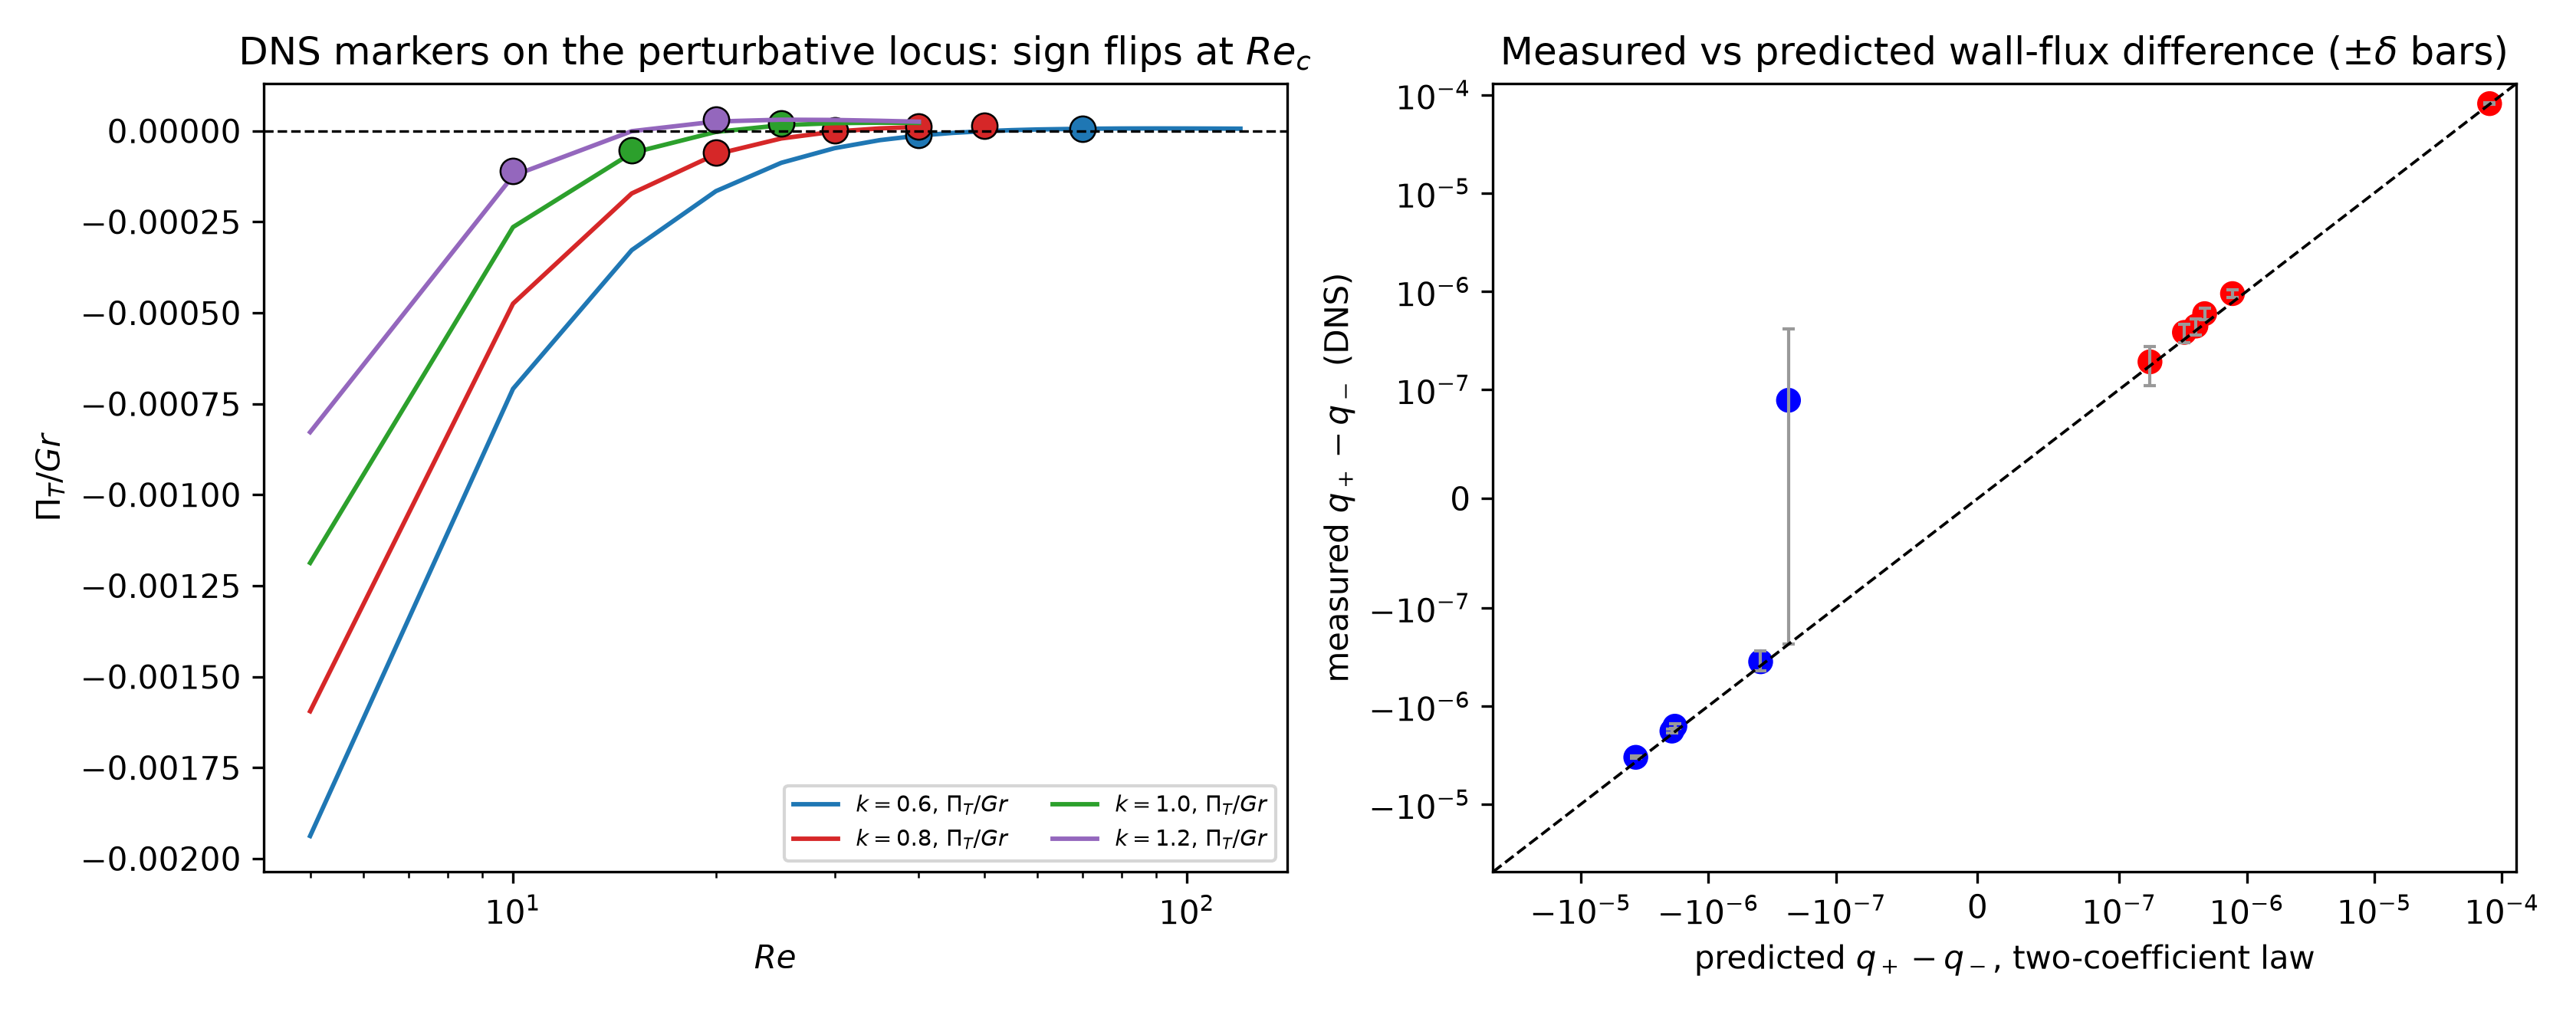
\includegraphics[width=0.98\textwidth]{campaign_v2_symmetry_selection/FIG_v2_10_dns_multik.png}
  \caption{(a)~Measured pumping coefficient divided by $\Grr$ (markers) against
  the perturbative locus (lines) at the four wavenumbers bracketed by
  DNS; every marker pair straddles its own $\Rey_c$ with opposite sign. This
  panel tests the direction of the reversal. (b)~Measured versus predicted
  wall-flux difference for the twelve non-degenerate
  runs, with error bars $2|\widehat\varepsilon_a\widehat\varepsilon_s^{\,*}|
  \delta_\Pi$. This panel tests the magnitude, and is the one the error model of
  Sec.~\ref{subsec:error_model} is judged against. Eleven of the twelve lie on
  the predicted side of zero; the outlier is the ladder run, the single case
  whose margin was below unity before the campaign was launched.}
  \label{fig:dns_multik}
\end{figure}

\subsection{What the campaign changes about the error model}
\label{subsec:error_model}

The campaign falsifies part of its own pre-registered error model. Of the twelve
non-degenerate cases, seven satisfy
$\delta_\Pi=\max(2.71\times10^{-4},1.52\%\,|\PiT|)$ and five exceed it, by up to
$4.6$ times. The pattern is systematic rather than random: the coefficient-space
deviation is independent of the forcing amplitude (item~3 above) and grows
monotonically with the wavenumber, its maximum over the bracket pairs rising
from $1.15\times10^{-4}$ at $k=0.6$ through $4.30\times10^{-4}$ at $k=0.8$ and
$7.47\times10^{-4}$ at $k=1.0$ to $1.25\times10^{-3}$ at $k=1.2$. Two consequences
follow. First, the $1.52\%$ figure quoted for the reference case is
specific to $(k,\Rey)=(0.8,10)$, where $|\PiT|$ is large; near a crossing the
relevant quantity is the absolute offset, not a relative one. Second, a DNS test
of the reversal at wavenumber $k$ is meaningful only for
$|\PiT(k,\Rey)|\gtrsim\delta_\Pi(k)$, which the bracket design of item~1
satisfies in every pair except the ladder run.

\subsection{What drives the growth of the remainder with $k$}
\label{subsec:remainder}

The monotone growth is the interesting part of the table, and it has two
candidate causes that this campaign does not separate. The first is physical:
the second-order truncation neglects harmonics $2k$ and $3k$ and the wall-normal
gradients grow with $k$, so a higher-order remainder is expected to increase
with the wavenumber. The deviation grows monotonically with $k$ over the four
resolved wavenumbers, and a log--log fit of the eight bracket runs gives
$|\Delta\PiT|\propto k^{3.4\pm1.7}$ at $R^2=0.84$ over the narrow span
$k=0.6$--$1.2$. That exponent is not statistically sharp enough to discriminate
between candidate higher-order mechanisms, so the growth is reported as an
empirical observation and not as a scaling law: no power of $k$ enters any
subsequent argument of this paper, and the separation of the growth from the
mesh-resolution floor is identified as future work below.
The second candidate is numerical, and it cannot be dismissed by the residuals
alone. The time-stepping and solver errors are genuinely negligible---the final
residuals are below $2.2\times10^{-8}$, four orders under the deviations they
accompany---but the spatial discretisation is not: on the published convergence
ladder at $k=0.8$, $\PiT$ moves by $3.1\times10^{-4}$ between the production
mesh of $3136$ degrees of freedom and the finest tested, $7008$, which is the
same order as the deviations measured here at $k=0.8$ and $k=1.0$. Because the
mesh is held at $N_x=64$ while the wavelength shrinks, a truncation error of
this kind predicts precisely the observed growth with $k$.

Two observations narrow the field. The deviation is amplitude-independent at
fixed $k$ (item~3), whereas a genuine higher power of the forcing would scale
with $\varepsilon^2$; the remainder is therefore either a mesh effect or a
$k$-dependent contribution that does not multiply $\widehat\varepsilon_a
\widehat\varepsilon_s^{\,*}$, such as the feedback of the second-order mean
field on the base temperature gradient. And the growth is confined to the
comparison with the perturbative coefficient: the \emph{sign} structure, which
is what the paper claims, is recovered in all eight bracket pairs. A decisive
separation requires one replica of the $k=1.2$ pair at refined $N_x$: if the
deviation collapses toward the floor, the growth is discretisation; if it
persists, it is the remainder of the truncation. That test is identified as
future work rather than asserted here.

Grashof-independence of the reversal point (Corollary~\ref{cor:Gr_independence})
is verified perturbatively to better than $10^{-9}$ in $\Rey_c$ and now
nonlinearly as well: DNS at the Grashof pair $(\Grr,\Rey)=(50,20)$, $(200,20)$,
$(50,50)$, $(200,50)$ returns Grashof ratios $4.0003$ and $4.0015$ with the
predicted sign preserved in both pairs
(Sec.~\ref{subsec:Gr_test}).

\section{Conclusions}
%--------------------------------------------------------------

This study separates what reflection symmetry forces from what the coupled
thermal--hydrodynamic dynamics choose. The organizing result is that the
\emph{structure} of the nonlinear wall-flux redistribution is fixed exactly by
symmetry, whereas its \emph{amplitude and sign} are dynamical, and that the
Reynolds number---even at fixed P\'eclet number---controls the direction of the
resulting thermal pumping.

\emph{What symmetry selects.} The first-order thermal fields decompose uniquely
into symmetric and antisymmetric parts; their hydrodynamic responses inherit
opposite reflection parities, so the mixed quadratic forcing is necessarily odd
across the channel. The second-order mean temperature correction is therefore
odd, which imposes
\begin{equation}
\boxed{
\Nu_{2,0}(+1) = -\Nu_{2,0}(-1)
}
\end{equation}
This is a structural consequence of the governing equations: it holds whether or
not the pumping amplitude is large, small, or zero.

\emph{What the dynamics select.} The redistribution is measured by the
thermal-pumping coefficient, for which the Green identity
$\PiT=-(\Pe/2)\int_{-1}^{1}Y\,\mathcal{E}_{as}\,dY$ yields
\begin{equation}
\PiT=\Grr\,A(k,\Rey,\Pr),
\qquad
A(k,\Rey,\Pr)=O(k^{2})\ \ \text{as}\ \ k\rightarrow0 .
\end{equation}
Linearity in $\Grr$ separates the buoyancy amplitude from the response, and the
long-wavelength limit shows that a slowly varying wall pattern cannot drive the
effect. Because $\PiT$ is proportional to $\Grr$, its zero is independent of
$\Grr$ (Corollary~\ref{cor:Gr_independence}): the reversal point is
$\Rey_c=30.8384965$ for $\Grr=25,50,100$ and $200$, with an absolute spread of
$1.2\times10^{-10}$ and $A$ invariant to better than $10^{-10}$ relative. DNS
reproduces the proportionality itself: at $\Rey=20$ and $\Rey=50$ the measured
Grashof ratio of $q_+-q_-$ is $4.0003$ and $4.0015$, and the sign predicted on
either side of the crossing survives.

\emph{Phase selects a second, independent coefficient.} Allowing a phase lag
$\phi$ between the two walls makes the mixed product complex, and streamwise
averaging leaves two independent invariants rather than one. The wall flux
becomes
\begin{equation}
\Nu_{2,0}(+1)=\Re(\varepsilon_a\varepsilon_s^{*})\,\PiT
+\Im(\varepsilon_a\varepsilon_s^{*})\,\PiT^{\perp},
\end{equation}
with $\PiT=-4.74850846\times10^{-2}$ and
$\PiT^{\perp}=+8.89496095\times10^{-2}$ at the reference state: the quadrature
coefficient is of opposite sign and nearly twice as large. For equal wall
amplitudes the in-phase invariant vanishes identically and the response obeys
$\Nu_{2,0}(+1)\propto\sin\phi$ exactly (Corollary~\ref{cor:sinphi}), verified phase
by phase to $2.4\times10^{-13}$. This is a selection rule, not a suggestion: it fixes which
combinations of wall forcing can pump and in which quadrature.

\emph{Reversal is systematic, and it is a magnitude race, not a phase flip.}
The reversal point has been mapped over seven wavenumbers, giving
$\Rey_c$ from $79.08$ at $k=0.4$ to $8.54$ at $k=2.0$; the reversal is resolved
at every wavenumber sampled, and its locus follows
$\Rey_c\approx21.50\,k^{-1.47}$ to within $11\%$ over that range. The DNS confirms the reversal at the
reference wavenumber: $\PiT^{\mathrm{DNS}}=-4.6763\times10^{-2}$, $1.52\%$ from
the perturbative $-4.7485\times10^{-2}$, with the sign change between
$\Rey=20$ and $\Rey=30$ at fixed $\Pe=7$ reproduced nonlinearly, and at three
further wavenumbers: all eight runs that bracket $\Rey_c$ at $k=0.6$, $0.8$,
$1.0$ and $1.2$ return the predicted sign, and the quadrature coefficient is
measured to $1.38\%$ (Sec.~\ref{sec:outlook}). The term-wise
decomposition of $\PiT$ shows what does \emph{not} happen: the antisymmetric
wall-normal transport term never crosses zero and the unwrapped phase lag
$\Delta\varphi^{(a)}$ increases monotonically from $-2.154$ to $-1.532$ rad
across the reversal. The sign change arises because the magnitudes of the
advective and wall-normal contributions become comparable
($|T_{Va}|/|T_{Ua}|$ falls from $3.40$ to $0.936$), with the subdominant
symmetric terms deciding the crossing to within $6\%$.

\emph{Independent nonlinear evidence.} DNS confirms the Grashof scaling
$\PiT\propto\Grr$ with a coefficient of determination effectively equal to unity
and a vanishing response at $\Grr=0$, recovers the reflection identity
$\PiT(\varepsilon_1,\varepsilon_2)=-\PiT(\varepsilon_2,\varepsilon_1)$, and
reproduces the exact cancellation of the parity limit: at equal wall amplitudes
and $\phi=0$ the two measured wall fluxes agree to $3.1\times10^{-18}$, against
individual fluxes of $1.15\times10^{-7}$, a relative precision of
$2.7\times10^{-11}$. On the Grashof pair of Sec.~\ref{subsec:Gr_test} the
nonlinear correction is itself proportional to $\Grr$, so it rescales the
coefficient without shifting its zero: Corollary~\ref{cor:Gr_independence}
survives beyond the perturbative regime.
Spatial and temporal refinement demonstrate convergence of the nonlinear
observable. The campaign also falsifies part of its own pre-registered error
model: five of the twelve non-degenerate cases exceed $\delta_\Pi$, with an
excess that is independent of the forcing amplitude and grows with the
wavenumber (Sec.~\ref{subsec:remainder}); separating the truncation remainder
from the residual spatial discretisation requires a refined-$N_x$ replica of
the $k=1.2$ bracket pair, which is the immediate next test. The remaining
finite-domain statement
$\Pe_c=10.871940554611$ is the value at which the zero set of $\PiT(k,\Pe)$
leaves the imposed interval $0.02\le k\le10$ at $\Rey=10$; it is a property of
the window, not an instability threshold.

Future work should extend the present approach beyond the two-dimensional
laminar setting: larger modulation amplitudes, three-dimensional configurations
and turbulent mixed convection. The most immediate testable consequence of the
two-coefficient law is the quadrature prediction of
Section~\ref{sec:outlook}---equal-amplitude forcing at $\phi=\pi/2$ gives
$\Nu_{2,0}(+1)=+4.0580\times10^{-5}$ in DNS against $+4.003\times10^{-5}$
predicted, whereas the in-phase-dominated forcing used in the earlier validation
gives $-7.123\times10^{-6}$; the two cases differ only
in $\Im(\varepsilon_a\varepsilon_s^{*})$. Wall-temperature phase and amplitude
asymmetry therefore constitute a control knob for the direction of thermal
pumping, with the Reynolds number setting where the knob changes sign.

\begin{acknowledgments}
{\sloppy
The author acknowledges the open-source scientific Python ecosystem, in particular NumPy, SciPy, and Matplotlib,
used for the numerical boundary-value, shooting, quadrature, and visualization calculations.
}
\end{acknowledgments}

\section*{Data availability}
All numerical data supporting this study, together with the manuscript source, the
supplementary document, the
scripts of the verification campaigns, the figures and this article's data package, are
openly deposited in a public repository at the address
\medskip

\noindent\mbox{\footnotesize\url{https://github.com/Ahmedalgeria778/symmetry_selected_thermal_pumping}}
\medskip

\noindent The
supplementary document carries the derivations and the supporting floats cited from the
text and numbered with an \textbf{S}; the data package itself gathers
64 files, documented item by item and inventoried with the size, line count and SHA-256
digest of every entry. Group A of that package holds the dense $\Pe$ survey behind
Fig.~\ref{fig:endpoint}; group B the perturbative reversal and phase campaigns of
Secs.~\ref{sec:reversal} and \ref{sec:phase}; group C the nonlinear DNS results of
Sec.~\ref{sec:dns_validation}, including the pre-run predictions, the raw per-case
measurements, the derived deviation table and the analysis summary of the confirmation
campaign of Sec.~\ref{sec:outlook}, the four-run Grashof-pair matrix of
Sec.~\ref{subsec:Gr_test} and the reduced data behind Fig.~\ref{fig:dns_grpair}; and group D
the boundary-value, shooting and analysis scripts that regenerate every table and figure
of this paper from the raw records. The DNS matrix runs from a single driver that
performs a dry run unless an explicit go-ahead flag is supplied and resumes from its own
checkpoint. The package inventory maps each figure and table of the paper to the files
that produce it.

%--------------------------------------------------------------%--------------------------------------------------------------
% Bibliography (single style already declared in the preamble)
\bibliography{references}

\end{document}
